


\chapter{Modelización Matemática de una Red Neuronal Convolucional} \label{ch:seccion12}

\noindent Nuestro primer objetivo será tratar de llegar a la modelización matemática de lo que es una \textbf{CNN}, para ello necesitamos en primer lugar definir un operador que denominaremos \textbf{propagador de dispersión} (PD) que será el que aplicaremos de forma recursiva en la cascada de convoluciones que modeliza una CNN, para ello explicaremos la problemática de elegir una operador \textit{lipschitz-continuo} bajo la acción de difeomorfismos e \textit{invariante por traslaciones}, para evitar problemas como las inestabilidades en altas frecuencias que se producen en las señales bajo la acción de difeomorfismos como ocurre si usamos el módulo de la transformada de Fourier. 

\medskip

\noindent Tras esto  veremos posibles alternativas para evitar que se produzcan estas inestabilidades, mediante el uso de bases de la transformada de ondeletas de \textbf{Littlewood-Paley}. En concreto con esta segunda alternativa obtendremos un operador que es \textbf{Lipschitz-continuo} bajo la acción de difeomorfismos. 

\medskip

\noindent Después, nuestra tarea será conseguir calcular coeficientes que sean invariantes por traslaciones, y para ello necesitaremos utilizar un operador no lineal como es el módulo. 

\medskip

\noindent Una vez tengamos un operador con todas las propiedades anteriores presentaremos el \textbf{PD}, y será la aplicación en cadena de este operador anterior sobre un \entrecomillado{camino} de frecuencias y rotaciones el que definirá la modelización matemática de una Red Neuronal Convolucional.


\section{De Fourier a las ondeletas de Littlewood-Paley}

\subsection{El módulo de la Transformada de Fourier}

\noindent El análisis de Fourier tradicionalmente ha jugado un papel fundamental en el procesamiento de señales \cite{DigitalImageProcessing}, por lo que podría parecer un buen punto de partida para la construcción del \textbf{propagador de dispersión} emplear la \textbf{transformada de Fourier}, una de las herramientas matemáticas más potentes en este campo. La intuición detrás de su fórmula es la de representar funciones no periódicas (pero que tienen área bajo la curva finita) como la integral de senos y cosenos multiplicados por una función que determina los pesos en cada instante. Formalmente tiene la siguiente expresión:

\begin{equation}
\widehat{f}(\omega):= \int{f(x)e^{-ix\omega}dx}=\int{f(x)\left[\cos{x\omega} -i\sin{x\omega}\right]dx}.
\end{equation}

\noindent Entre las propiedades más destacables de la transformada encontramos el hecho de que una función se puede recuperar sin pérdida de información a partir de su transformada de Fourier, lo cual nos permite poder trabajar en el \entrecomillado{Dominio de Fourier}\footnote{También llamado \entrecomillado{Dominio de Frecuencia}} ya que al calcular la integral, la función resultante sólo depende de $\omega$ (la frecuencia), y posteriormente pasar de nuevo al dominio original de la función, aplicando la inversa de la transformada sin pérdida de información.

\medskip

\noindent Esto a priori es algo atractivo, pues nos permitiría trabajar en un dominio más sencillo y extraer conclusiones que podemos traducir al dominio original de la señal sin pérdida de información. Además, en el estudio de señales se suele emplear el módulo de la transformada de Fourirer para evitar fases complejas en el análisis, de esta forma el operador que vamos a probar en primer lugar es: 

\begin{definicion}
$\Phi(f)=|\widehat{f}|$ módulo de la transformada de Fourier. 
\end{definicion}

\noindent Vamos a comprobar si se trata de un operador válido para nuestro propósito. Para ello necesitamos en primer lugar que sea un operador \textbf{Invariante por traslaciones}. Veamos  que sí cumple esta propiedad.

\begin{lema} \label{lema::invarianza_traslaciones}
    El operador $\Phi(f)=|\widehat{f}|$ es invariante por traslaciones.
\end{lema}

\begin{proof}
    \noindent Para ello tenemos que ver que si definimos para cada $c \in \mathbb{R}^d$, la traslación $L_cf(x)=f(x-c)$ se tiene que :  
    
    $$\widehat{L_cf}(w)=\int_{\mathbb{R}^d}{L_cf(x) e^{-ixw} dx}=\int_{\mathbb{R}^d}{f(x-c)e^{-ixw}dx}$$
    
    \noindent Y realizando el cambio de variable $x-c=y$ se tendría que: 
    
    \begin{align*}
        \int_{\mathbb{R}^d}{f(x-c)e^{-ixw}dx} &= \int_{\mathbb{R}^d}{f(y)e^{-i(y+c)w}dy}= \\      &=\int_{\mathbb{R}^d}{f(y)e^{-iyw}e^{-icw}dy}= \\ &=\int_{\mathbb{R}^d}=e^{-icw}\int_{\mathbb{R}^d}{f(y)e^{-iyw}dy}=e^{-icw}\widehat{f}(w)
    \end{align*}
    
    \noindent Por lo que se tiene que $|\widehat{L_cf}(w)|=|e^{-icw}| |\widehat{f}(w)|=|\widehat{f}(w)|$ y entonces $\Phi(f)=|\widehat{f}|$ es invariante a traslaciones. \qedhere
\end{proof}

\medskip
    
\noindent Sin embargo, la invaianza por traslaciones no es suficiente, necesitamos también que nuestro operador sea invariante frente a pequeñas deformaciones (difeomorfismos). De esta forma, un operador $\Phi(f)$ diremos que es estable frente a deformaciones si verifica \autoref{def::Lipschitz_cont}. Sin embargo, esta propiedad no la verifica el módulo de la transformada de Fourier, como podemos ver a continuación:

\begin{observacion}\label{lemma:TF_inestable_difeomorfismos}
  El módulo de la Transformada de Fourier no es estable frente a pequeñas deformaciones y no es \entrecomillado{Lipschitz-continuo} en el sentido de la \autoref{def::Lipschitz_cont}.

  \medskip

  \noindent Si consideramos la función $\tau(x)\coloneqq \epsilon x$ con $0 < \epsilon << 1$. De esta forma $||\nabla \tau (x) ||_\infty = \epsilon$ y $||H\tau(x)||_\infty=0$ con esto, la condición de Lipschitz para el módulo de la transfomada de Fourier nos daría la existencia de una constante $c>0$ de modo que la desigualdad que se tendría que cumplir para cada $f \in L^2(\mathbb{R}^d)$ y cada $0 < \epsilon << 1$ sería:

  $$\left|\left| \; |\widehat{f}| -|\widehat{L_\tau f}| \; \right|\right| \leq c ||f|| (||\nabla \tau ||_{\infty} + ||H\tau||_\infty) \leq c ||f|| \epsilon$$

  \noindent Vamos a ver un contraejemplo con una función de una dimensión por simplicidad.

  \medskip

  \noindent Supongamos que tenemos $f(x)=e^{i \xi x}e^{-|x|}$ donde $\xi$ está por determinar. Calculamos ahora $|\widehat{f}|$ y $|\widehat{L_\tau f}|$ teniendo en cuenta que :


  \begin{align*}
    |\widehat{f}(\omega)|&=\left|  \int{f(x)e^{-ix\omega}dx}  \right | \\
    &=\left|  \int{f(x)e^{-ix\omega}dx}  \right | \\
    &=\left|  \int{e^{i \xi x}e^{-|x|}e^{-ix\omega}dx}  \right | \\
    &=\left|  \int{e^{-ix(\xi-\omega)}dx}  \right | \\
    &=\left|  \int{e^{-|x|}\left[\cos{x(\xi-\omega)} -i\sin{x(\xi-\omega)}\right]dx} \right| \\
  \end{align*}

  \noindent En el último paso podemos descomponer la integral en suma de dos, y para simplificar las operaciones llamamos $\beta=(\xi - \omega)$. Así, aplicando las siguientes fórmulas conocidas para el cálculo de integrales,


  \begin{equation} \label{eq:res_auxiliar_1}
    \int_\mathbb{R} \cos(\beta x) e^{-|x|} dx= \frac{1}{1+\beta^2}
  \end{equation}

  \noindent y 

  \begin{equation}\label{eq:res_auxiliar_2}
    \int_\mathbb{R} \sin(\beta x) e^{-|x|} dx= 0
  \end{equation}

  \noindent a nuestro caso concreto, obtenemos que: 

  \begin{align*}
    |\widehat{f}(\omega)|&=\left|  \int{\cos{x\beta}e^{-|x|} dx} - i \int{\sin{x\beta}e^{-|x|} dx} \right| \\
    &=\frac{1}{1+\beta^2} \\
    &=\frac{1}{1+(\xi - \omega)^2}.
  \end{align*} 

  \noindent Ahora pasamos a calcular $|\widehat{L_\tau f}|$:

  \begin{align*}
    |\widehat{L_\tau f}(\omega)| &= |\widehat{f}((1-\epsilon)\omega)| \\
    &=\left|  \int{f((1-\epsilon)x)e^{-ix\omega}dx}  \right | \\
    &=\left|  \int{e^{i \xi (1-\epsilon) x}e^{-|(1-\epsilon)x|}e^{-ix\omega}dx}  \right |. \\
  \end{align*}

  \noindent Ahora realizamos el siguiente cambio de variable

  \begin{equation}
    \tilde{x}=(1-\epsilon) x \implies x=\frac{\tilde{x}}{1-\epsilon} 
  \end{equation}

  \begin{equation}
  d\tilde{x}=(1-\epsilon) dx \implies dx=\frac{1}{(1-\epsilon)}d\tilde{x}
  \end{equation}

  \noindent y aplicando los cambios a lo que teníamos nos queda

  \begin{align*}
    |\widehat{L_\tau f}(\omega)| 
    &= \frac{1}{(1-\epsilon)}\left|  \int{f((1-\epsilon)x)e^{-ix\omega}dx}  \right | \\
    &=\frac{1}{(1-\epsilon)}\left|  \int{e^{i \xi \tilde{x}}e^{-|\tilde{x}|}e^{-i\frac{\tilde{x}}{(1-\epsilon)}\omega}d\tilde{x}}  \right | \\
    &=\frac{1}{(1-\epsilon)}\left|  \int{e^{i \left[ \frac{(1-\epsilon) \xi - \omega}{(1-\epsilon)}\right]\tilde{x}}e^{-|\tilde{x}|} d\tilde{x}}  \right | \\
    &=\frac{1}{(1-\epsilon)}\left|  \int{e^{i \tilde{\beta}\tilde{x}}e^{-|\tilde{x}|} d\tilde{x}}  \right |, \\
  \end{align*}

  \noindent como podemos ver, llegamos a una integral que se resuelve de la misma manera que en el caso anterior haciendo uso de \eqref{eq:res_auxiliar_1} y \eqref{eq:res_auxiliar_2}:

  \begin{align*}
    |\widehat{L_\tau f}(\omega)| 
    &= \frac{1}{(1-\epsilon)} \frac{1}{1+\tilde{\beta}^2} \\
    &= \frac{1}{(1-\epsilon)} \frac{1}{1+\left[ \frac{(1-\epsilon) \xi - \omega}{(1-\epsilon)}\right]^2}. \\
  \end{align*}


  \noindent De esta forma hemos obtenido que para nuestro caso concreto de $f(x)=e^{i \xi x}e^{-|x|}$ ,


  \begin{align*}
    \left\| |\widehat{L_\tau f}|-|\widehat{f}| \right\| &= \left\| \frac{1}{(1-\epsilon)} \frac{1}{1+\left[ \frac{(1-\epsilon) \xi - \omega}{(1-\epsilon)}\right]^2}-\frac{1}{1+(\xi - \omega)^2} \right\| \\
    &\geq  \left\| \frac{1}{1+\left[ \frac{(1-\epsilon) \xi - \omega}{(1-\epsilon)}\right]^2}-\frac{1}{1+(\xi - \omega)^2} \right\| \\
    &=\left(\int_{\mathbb{R}} \left| \frac{1}{1+\left[ \frac{(1-\epsilon) \xi - \omega}{(1-\epsilon)}\right]^2}-\frac{1}{1+(\xi - \omega)^2} \right|^2 d\omega\right)^{1/2}.
  \end{align*}


  \noindent A continuación vamos a intentar aproximar el valor del módulo de la integral, para ello en primer lugar vamos a realizar el siguiente cambio de variable 

  \begin{align*}
    &t=\omega-\xi \implies \omega-(1-\epsilon)\xi= \omega-\xi + \epsilon\xi = t +\epsilon\xi \\
    &dt=d\omega.
  \end{align*}

  \noindent Así, obtenemos que: 

  \begin{align*}
    \int_{\mathbb{R}} \left| \frac{1}{1+(\xi - \omega)^2} - \frac{1}{1+\left[ \frac{(1-\epsilon) \xi - \omega}{(1-\epsilon)}\right]^2} \right|^2 d\omega &\geq
    \left|\int_{\mathbb{R}} \left(  \frac{1}{1+(\xi - \omega)^2} - \frac{1}{1+\left[ \frac{(1-\epsilon) \xi - \omega}{(1-\epsilon)}\right]^2}  \right)^2 d\omega \right| \\
    &=\left|\int_{\mathbb{R}} \left(  \frac{1}{1+t^2} - \frac{1}{1+\left[ \frac{t+\epsilon\xi}{(1-\epsilon)}\right]^2}  \right)^2 d\omega \right| \\
  \end{align*}

  \noindent Representando la gráfica $g_1(t)= \frac{1}{1+t^2}$, podemos ver cómo el valor de su integral se acumula en torno al origen de coordenadas, y en cambio $g_2(t)=\frac{1}{1+\left[ \frac{t+\epsilon\xi}{(1-\epsilon)}\right]^2}$ e una traslación y escalado de la función anterior. De esta forma, si $\epsilon\xi$ es muy grande, el área de la función $g_2(t)$ será prácticamente cero en la región del espacio dónde $g_1(t)$ concentra su integral. Dicho de otra forma, las dos funciones tendrían soporte disjunto.

  \noindent De esta forma, podemos tomar una constante $M>0$ tal que para un valor de $\xi$ elevado se cumpla que: 

  \begin{align*}
    \int_{\mathbb{R}} \left| \frac{1}{1+(\xi - \omega)^2} - \frac{1}{1+\left[ \frac{(1-\epsilon) \xi - \omega}{(1-\epsilon)}\right]^2} \right|^2 d\omega 
    &\geq \int_{-M}^{M} (g_1(t)-g_2(t))^2 dt \\
    &\approx \int_{-M}^{M} g_1(t)^2 dt. \\
  \end{align*}

  \noindent Y como $\xi$ puede ser arbitrariamente grande, intuitivamente el intervalo en el que ambas funciones tienen soporte disjunto crece de forma indefinida lo cual nos permite realizar la siguiente aproximación teniendo en cuenta que $g_1(t)=\widehat{f}$:

  \begin{equation} \label{eq::1.1}
    \left\| |\widehat{f}| -|\widehat{L_\tau f}| \; \right\| \sim \|g_1(t) \|=\|f\|. 
  \end{equation}

  \noindent Dónde la última igualdad la hemos realizado gracias a la fórmula de Plancharel que en el caso de $\mathbb{R}^d$ es: 

  \begin{equation} \label{eq::Plancharel}
    \int_{\mathbb{R}^d} \left|f(x)\right|^2 dx= \int_{\mathbb{R}^d}\left|\widehat{f}(\omega)\right|^2 d\omega.
  \end{equation}

  \noindent Luego hemos demostrado que en este caso particular el operador $|\widehat{f}|$ no cumple la condición de Lipschitz, pues como hemos mencionado antes, $\xi$ puede ser arbitrariamente grande y de esta forma, que la diferencia anterior pueda ser todo lo grande que se quiera.

  \begin{figure}[!h]
    \centering
    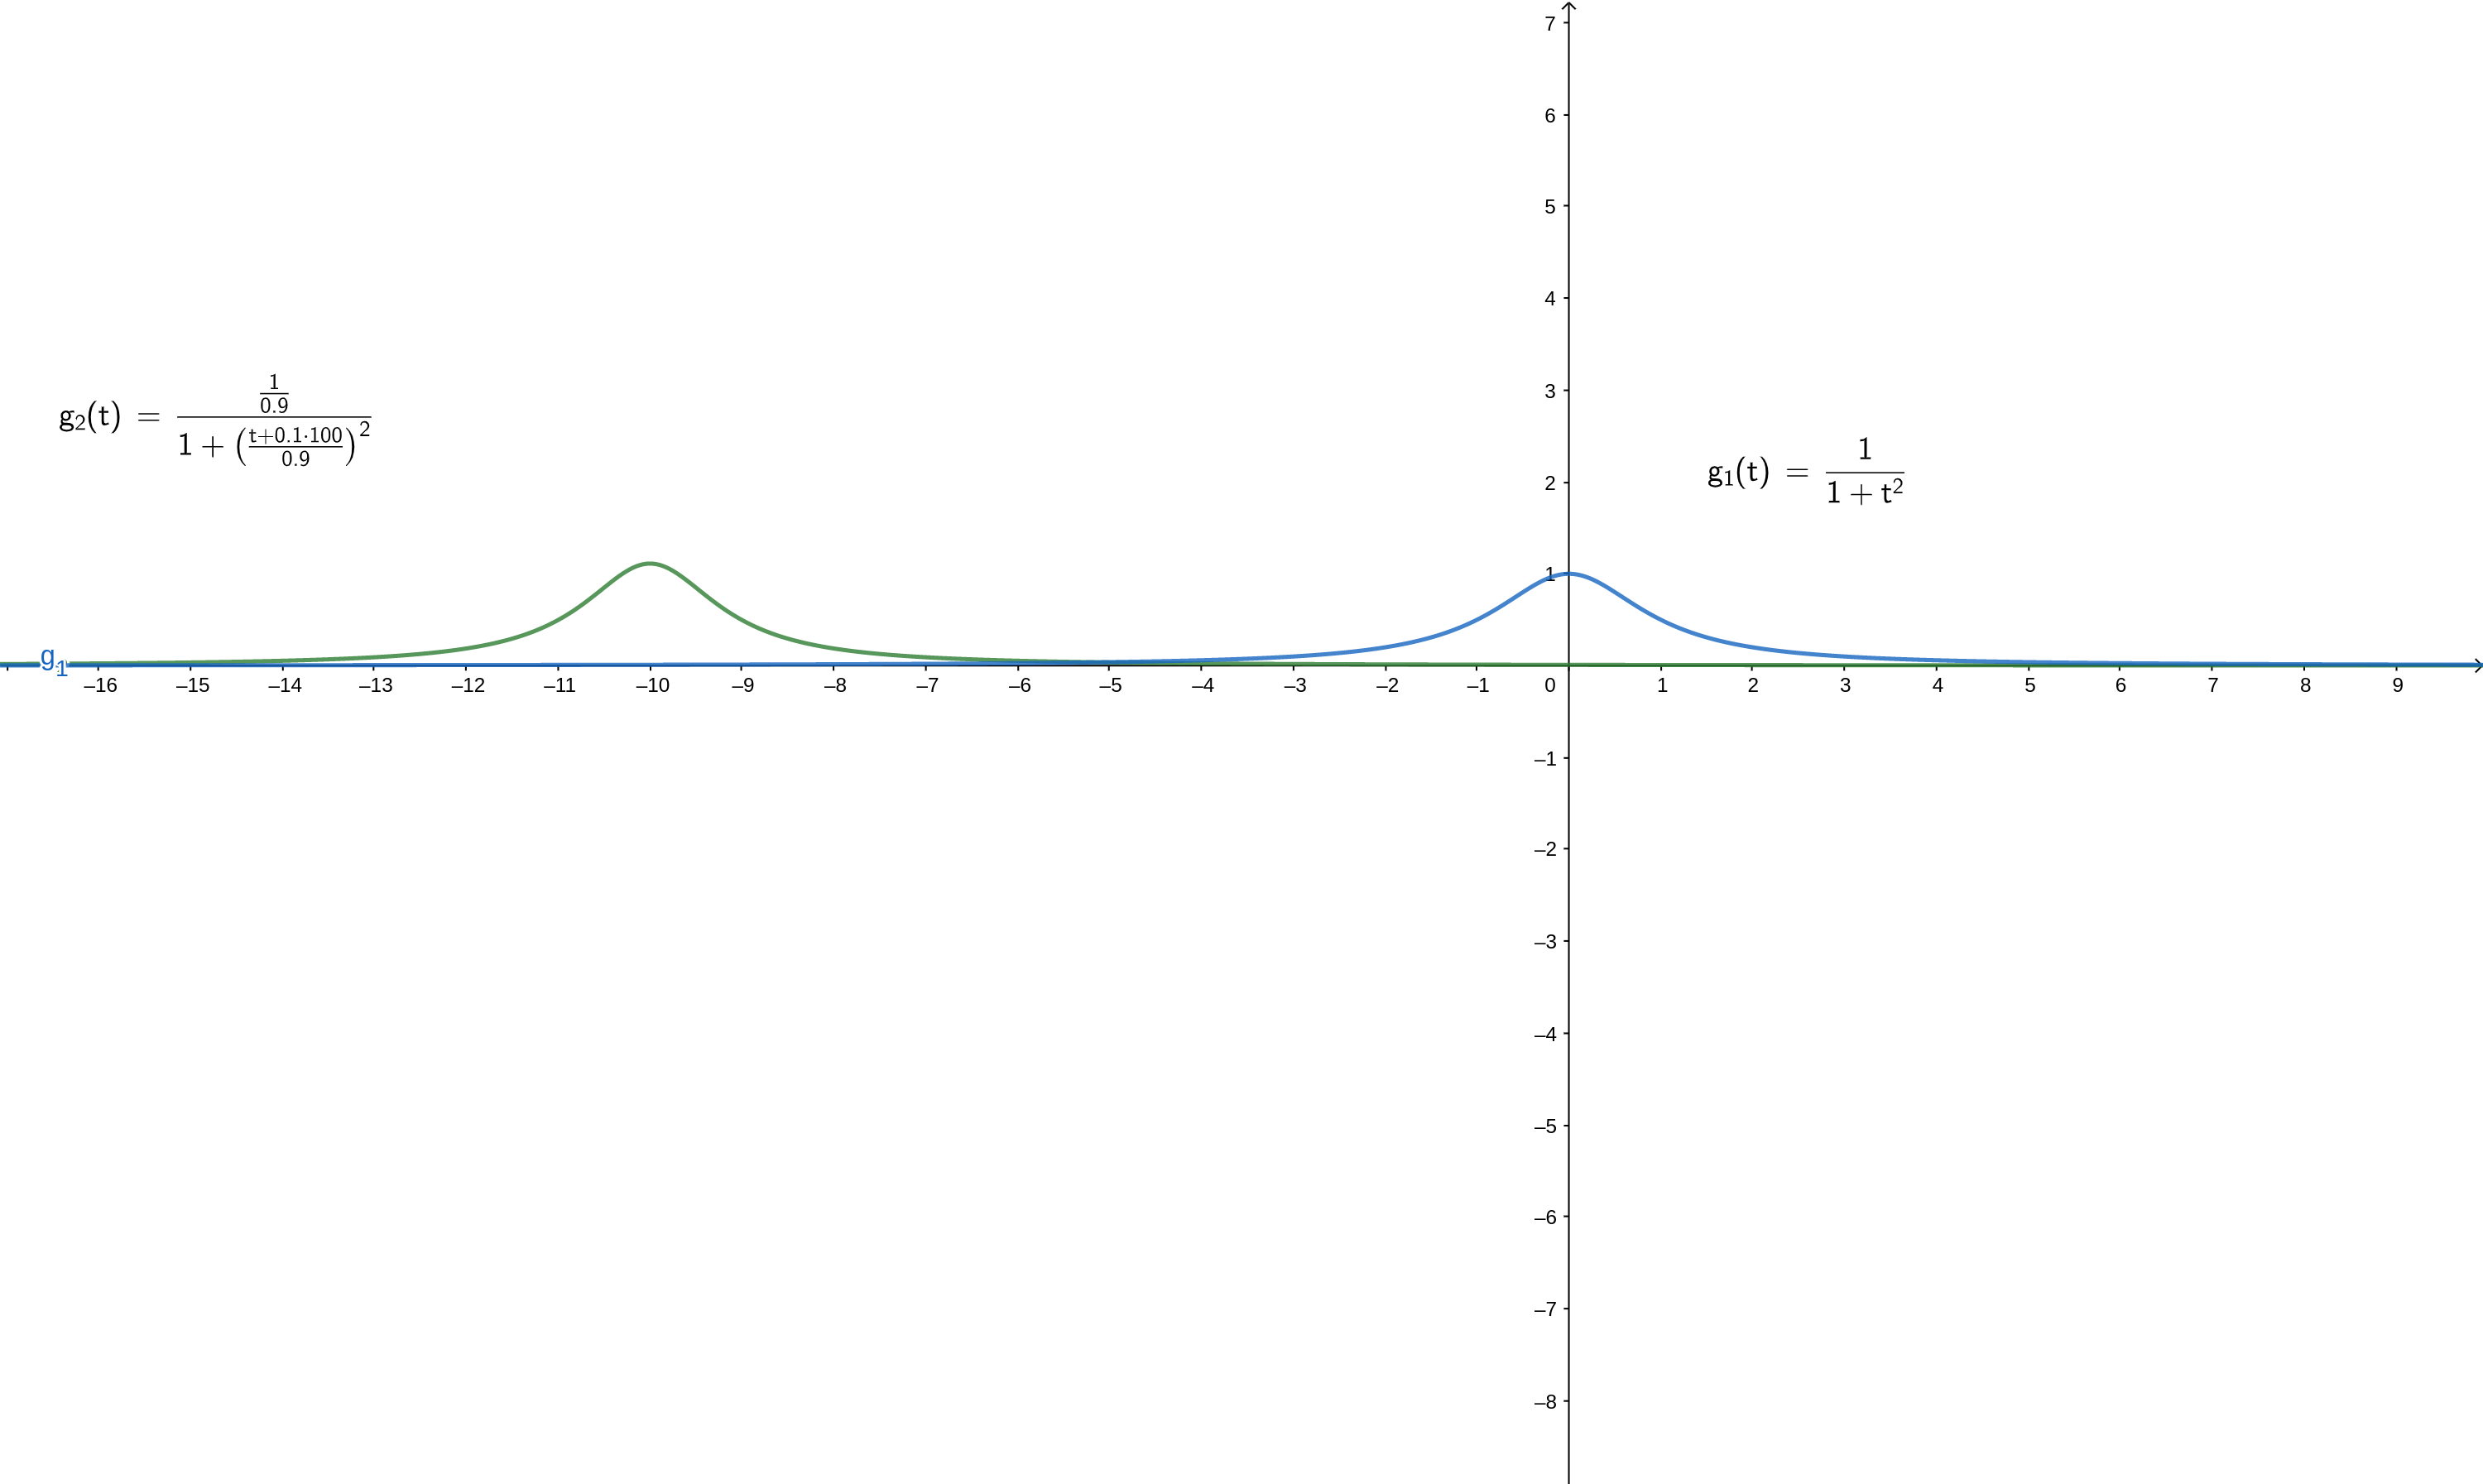
\includegraphics[width=1.0\textwidth]{img/geogebra-export_contraejemplo_Fourier.png}
    \caption{Como podemos ver en la imagen, para los valores $\epsilon=0.1$, $\xi=100$ y $M=5$ ambas funciones tienen soporte casi disjunto de manera que la diferencia entre ellas en el intervalo $[-5,5]$ coincide prácticamente con la integral de $g_1(t)$.}
    \label{fig:Grafica_funciones}
  \end{figure}

\end{observacion}
 
\medskip

\noindent Por esto, lo que haremos será reemplazar las ondas sinusoidales de la transformada de Fourier por funciones localizadas con un soporte mayor en altas frecuencias que nos permitan evitar estas complicaciones, que tendrán un mejor rendimiento en nuestro propósito. Estas funciones se denominan \textbf{ondeletas}. 

\medskip

\subsection{Alternativa: Las ondeletas}

\noindent Las ondeletas \cite{MallatWavelets} son pequeñas ondas estables bajo la acción de deformaciones, al contrario que las ondas sinusoidales de Fourier. Definiremos la transformada de ondeletas y veremos que calcula, mediante convoluciones con bases de ondeletas, coeficientes estables bajo la acción de difeomorfismos.

\medskip

\noindent Al contrario que las bases de Fourier, las bases de ondeletas definen  representaciones dispersas de señales regulares a trozos, que podrían incluir transiciones y singularidades. En las imágenes, los mayores coeficientes de las ondeletas se localizan en el entorno de las esquinas y en las texturas irregulares.

\medskip

\noindent A modo de ejemplo vamos a ver la base de Haar que, aunque no sea la que utilicemos para construir nuestro propagador de dispersión, puede ayudar a entender mejor la filosofía de las ondeletas. Se construye a partir de la siguiente función: 

$$ \psi(t)= \begin{cases} 
      1 & 0\leq t < 1/2 \\
      -1 & 1/2\leq t < 1 \\
      0 & \; en \; otro \; caso
   \end{cases}$$

\begin{figure}[!h]
  \centering
  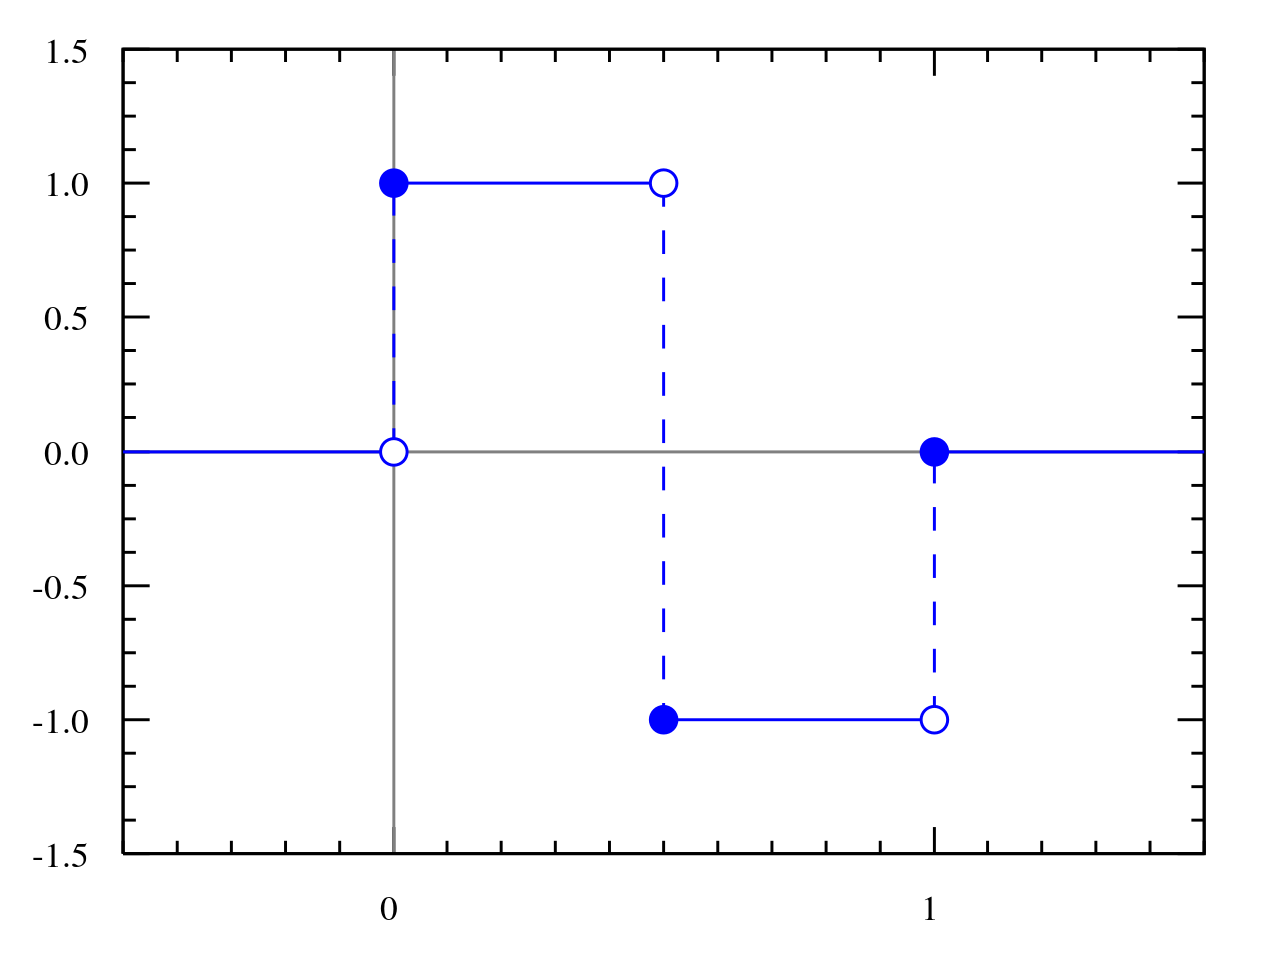
\includegraphics[width=0.5\textwidth]{img/Haar_wavelet.png}
  \caption{Representación gráfica de la ondeleta de Haar.}
  \label{fig:Ondeleta_de_Haar}
\end{figure}

\noindent A esta ondeleta la denominamos \textbf{ondeleta Madre}, pues a partir de ella, podemos generar la siguiente base ortonormal

\medskip

$$\left \lbrace \psi_{j,n}(t)= \frac{1}{\sqrt{2^j}} \psi\left(\frac{t-2^jn}{2^j}\right) \right\rbrace_{(j,n) \in \mathbb{Z}^2}$$

\noindent del espacio $L^2(\mathbb{R})$ de señales con energía finita.

\noindent Así, cualquier señal $f$ de energía finita puede ser representada por los coeficientes que se obtienen mediante el producto interno en $L^2(\mathbb{R})$ con la base anterior: 

$$\langle f,\psi_{j,n} \rangle =\int_{-\infty}^{+\infty} f(t) \psi_{j,n} (t) dt  $$

\noindent y puede recuperarse sumando en su base ortonormal:

$$f=\sum_{j=-\infty}^{+\infty}\sum_{n=-\infty}^{+\infty}  \langle f,\psi_{j,n} \rangle \psi_{j,n} $$

\noindent Esto nos permite (igual que pasaba con el módulo de la Transformada de Fourier) trabajar en un dominio más sencillo que nos permite procesar la información con mayor rapidez y posteriormente reconstruir la señal a partir de los coeficientes sin perder información. Algunas propiedades de la base de Haar serían: 

\newpage

\begin{itemize}
  \item Cada ondeleta $\psi_{j,n}$ tiene media $0$ en su soporte $[2^jn, 2^j(n+1)]$.
  \item Si $f$ es localmente regular y $2^j$ es próximo a $0$, entonces su intervalo con soporte es muy pequeño, debido a las propiedades de $f$, la función en el intervalo  $[2^jn, 2^j(n+1)]$ será prácticamente constante, lo que se traduce en que  y su coeficiente de ondeleta $\langle f,\psi_{j,n} \rangle$ es prácticamente cero.
  \item Los mayores coeficientes se localizan en los cambios bruscos de intensidad de señal, como pueden ser los bordes, las esquinas o las texturas en las imágenes, pues en estos casos somos capaces de encontrar un elemento de la base de Haar con cuyo soporte esté en el intervalo dónde se produzca el cambio de intensidad, y por lo tanto que tenga un coeficiente de ondeletas distinto de cero.
\end{itemize}

\noindent Para el caso concreto de imágenes \footnote{ver por ejemplo sección 1.1 de \cite{MallatWavelets}}, las bases de ondeletas ortonormales pueden construirse a partir de bases ortonormales en señales de una dimensión.Lo haremos a partir de tres ondeletas para capturar las variaciones horizontales, verticales y diagonales presentes en la imagen. Así, denominamos a las ondeletas usadas como $\psi^1(x)$, $\psi^2(x)$ y$\psi^3(x)$ con $x=(x_1,x_2)\in \mathbb{R}^2$, dilatadas por el factor $2^j$ y trasladadas por $2^jn$ con $n=(n_1,n_2) \in \mathbb{Z}^2$, se construye una base ortonormal para el espacio $L^2(\mathbb{R}^2)$: 
$$\left \lbrace \psi_{j,n}^k(x)= \frac{1}{\sqrt{2^j}} \psi^k\left(\frac{x-2^jn}{2^j}\right) \right \rbrace_{(j,n) \in \mathbb{Z}^2}$$

\medskip

\noindent El soporte de la ondeleta $\psi_{j,n}^k(x)$ es un cuadrado proporcional a la escala $2^j$ como podemos ver en la \autoref{fig:base_haar}. Las bases de ondeletas en dos dimensiones se discretizan para definir bases ortonormales de imágenes de N píxeles.


\begin{figure} [!h]
  \centering
  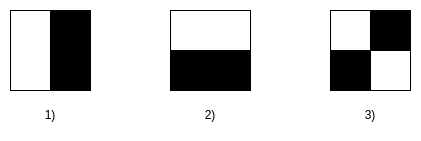
\includegraphics[width=0.8\textwidth]{img/base_haar_2d.png}
  \caption{En el ejemplo $1$ y $3$ podemos ver ejemplos de soportes para ondeletas especializadas en la detección de líneas verticales, en la imagen $2$ podemos ver un ejemplo de soporte de una ondeleta en el caso de la detección de líneas horizontales, y en el ejemplo $4$ para las diagonales. Todas tienen soporte cuadrado.}
  \label{fig:base_haar}
\end{figure}

\noindent Del mismo modo que en una dimensión, los coeficientes de ondeletas $\langle f,\psi_{j,n}^k \rangle$ serán pequeños si $f(x)$ es regular, y serán grandes cerca de los cambios bruscos de frecuencias como en los bordes o esquinas de las imágenes, como podemos ver en \autoref{fig:ejemplo_haar}. Los filtros resaltan los bordes en tres direcciones, horizontal (derecha) vertical (abajo) y en diagonal (abajo derecha).

\begin{figure} [!h]
  \centering
  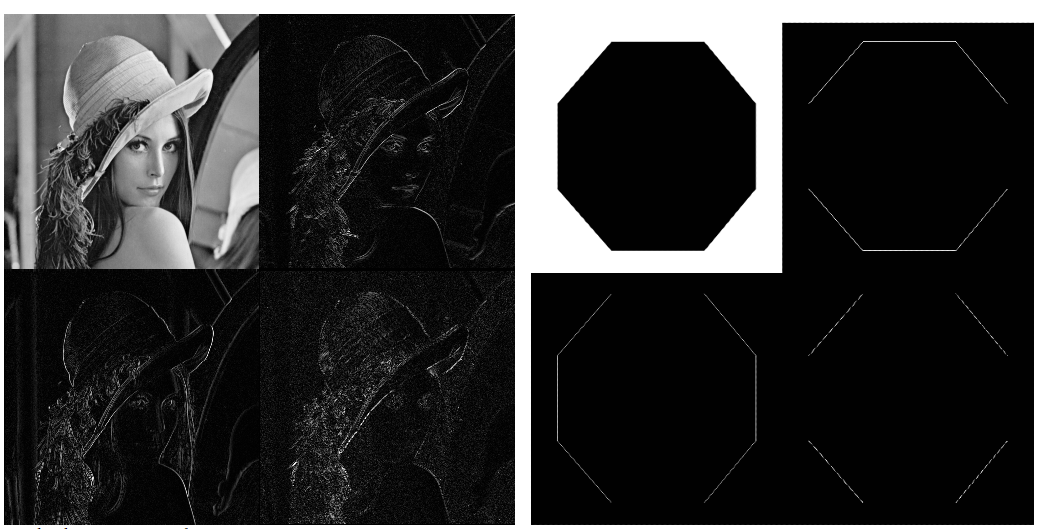
\includegraphics[width=0.8\textwidth]{img/ejemplos_haar_basis.png}
  \caption{Ejemplos de aplicar la base de Haar a dos imágenes \cite{HaarBasis}.}
  \label{fig:ejemplo_haar}
\end{figure}

\medskip 

\noindent Volviendo al propósito de definir el propagador de dispersión, la ondeleta madre que elijamos y la base ortogonal que forme se verán afectadas normalmente por escalados y rotaciones, por lo tanto definimos: 

\begin{definicion}
  Una ondeleta madre escalada por un factor $2^{-j}$ con $j \in \mathbb{Z}$ y rotada por $r \in G$ siendo $G$ el grupo finito de rotaciones, se escribe: 

  $$\psi_{2^j r}(x)=2^{dj} \psi(2^j r^{-1} x).$$
\end{definicion}


\medskip

\noindent Su transformada de Fourier es $\widehat{\psi_{2^j r}}(\omega)=\widehat{\psi}(2^j r^{-1} \omega)$.

\medskip

\noindent La transformada de dispersión que usaremos tendra una base de ondeletas generada por una ondeleta madre del tipo:

$$\psi(x)=e^{i\eta x} \Theta(x)$$

\noindent Donde $\widehat{\Theta}(x)$ es una función real centrada en una bola de baja frecuencia en $x=0$, cuyo radio es del orden de $\pi$.

\medskip

\noindent Y como podemos ver:

\begin{equation}
  \widehat{\psi}(\omega)=\int_{\mathbb{R}^d}e^{i \eta x} \Theta(x) e^{-i\omega x} dx=\int_{\mathbb{R}^d}\Theta(x) e^{ix(\omega-\eta)} dx=\widehat{\Theta}(\omega-\eta).
\end{equation}

\medskip

\noindent Por lo tanto, $\widehat{\psi}(\omega)$ es real y centrada en una bola de mismo radio pero centrada en $\omega=\eta$ que tras el escalado y rotación: 
$$\widehat{\psi}_\lambda(\omega)= \widehat{\Theta} (\lambda^{-1}\omega-\eta),$$ 

\noindent donde $\lambda=2^jr \in 2^{\mathbb{Z}}\times G$. 

\noindent Por lo tanto $\widehat{\psi}_\lambda(\omega)$ recubre una bola centrada en $\lambda^{-1}\eta$ con radio proporcional a $|\lambda|=2^j$.
 
\medskip 

\subsection{La Transformada de Littlewood-Paley}

\noindent Una vez conocemos un poco más en profundidad las ondeletas y su funcionamiento, pasamos a presentar la \textbf{Transformada de ondeleta de Littlewood-Paley}, que es la que emplearemos para construir el propagador de dispersión.

\medskip

\noindent Se trata de una representacion redundante que calcula convoluciones para todo $x \in \mathbb{R}^d$ sin realizar sub-muestreo: 

\begin{equation}
  \forall x \in  \mathbb{R}^d \;\; W[\lambda]f(x)= f \ast \psi_\lambda(x)=\int f(u)\psi_\lambda(x-u) du .
\end{equation}

\noindent Dónde $\ast$ denota la operación de convolución. 

\medskip

\noindent Calculamos su transformada de Furier, para ello tendremos en cuenta el teorema de Convolución de la Transformada de Fourier, el cual dice: 

\begin{teorema} \label{Teorema::Convolucion}
 Sean $f$ y $g$ dos funciones integrables.

 Si 

 $$h(x)=(f\ast g)(x)=\int f(y)g(x-y) dy$$

 Entonces: 

 $$\widehat{h}(\omega)=\widehat{f}(\omega) \widehat{g}(\omega)$$

 y 

 $$h(x)=(f \ast g)(x)= \int \widehat{f}(\omega) \widehat{g}(\omega) e^{-i\Omega x} d\omega$$
 
\end{teorema}

De esta manera, se tiene que: 

$$\widehat{W[\lambda]f(\omega)}=\widehat{f}(\omega)\widehat{\psi_\lambda}(\omega)=\widehat{f}(\omega)\widehat{\psi}(\lambda^{-1}\omega).$$

\noindent Además, teniendo en cuenta la propiedad que nos dice que si la función $f$ es real, entonces su transformada coincide con el conjugado complejo $\widehat{f}(-\omega)=\overline{\widehat{f}(\omega)}$ podemos ver que: 

\begin{itemize}
  \item si $\widehat{\psi}(\omega)$ y $f$ son reales entonces $W[-\lambda]f= \overline{W[\lambda]f}$, utilizando la misma propiedad de antes. Además, si denotamos por $G^{+}$ al cociente de G con $\lbrace-\mathbb{1},\mathbb{1}\rbrace$, conjunto en el cual las dos rotaciones $r$ y $-r$ son equivalentes, sería suficiente calcular $W[2^jr]f$ para las rotaciones "positivas" de $G^{+}$.
  \item En cambio, si $f$ fuese compleja, entonces $W[2^jr]f$ tendría que calcularse para todo $r \in G$.
\end{itemize}

\medskip
 
\noindent La transformada de Littlewood-Paley a una cierta escala $2^J$ sólo mantiene las ondeletas de frecuencias $2^j>2^{-J}$ pues el resto de ondeletas de la base no tendrían soporte. De esta forma, las bajas frecuencias que no son cubiertas por estas ondeletas vienen dadas por un promedio en el dominio proporcional a $2^J$:

\begin{equation}
  A_Jf=f \ast \phi_ {2^J} \; \; con \; \phi_ {2^J}(x)=2^{-dJ} \phi(2^{-J}x).
\end{equation}

\medskip

\noindent Así, si $f$ fuese real, entonces la transformada de ondeleta tendría la siguiente expresión: 

$$W_J f=\lbrace A_Jf,(W[\lambda]f)_{\lambda \in \Lambda_J} \rbrace$$ 

\noindent Es decir, estaría formada por el promedio de todas las odeletas de la base que no tienen soporte a la escala fijada $2^J$, y el conjunto de coeficientes producidos al convolucionar cada elemento de la base con $2^j>2^{-J}$ con la señal $f$. Para denotar esto indexamos por $\Lambda_J=\lbrace \lambda=2^jr:\;r\in G^{+}, \; 2^j>2^{-J}\rbrace$. 

\medskip

\noindent Su norma sería: 

\begin{equation}
  ||W_Jf||^2=||A_Jf||^2+\sum_{\lambda \in \Lambda_j} ||W[\lambda]f||^2.
\end{equation}

\medskip
 
\noindent Si $J=\infty$ entonces todas las ondeletas de la base obtendrían coeficientes no nulos y por lo tanto 
$$W_\infty f=\lbrace W[\lambda]f\rbrace_{\lambda \in \Lambda_\infty},$$ 

\noindent con $\Lambda_\infty=2^\mathbb{Z} \times G^{+}$. 

\noindent Su norma en este caso sería 

$$||W_\infty f||^2=\sum_{\lambda \in \Lambda_\infty} ||W[\lambda]f||^2.$$

\noindent En el caso en que $f$ sea compleja, se incluyen todas las rotaciones $W_Jf=\lbrace A_J f,(W[\lambda]f)_{-\lambda,\lambda \in \Lambda_J} \rbrace$ y $W_\infty f=\lbrace W[\lambda]f\rbrace_{-\lambda,\lambda \in \Lambda_\infty}$. 

\medskip

\noindent La siguiente proposición da una condición estándar de Littlewood-Paley para que $W_J$ sea unitario.

\begin{proposicion} \label{unitario}
 Para cualquier $J \in \mathbb{Z}$ o $J=\infty$, $W_J$ es unitario en el espacio de funciones reales o complejas de $L^2(\mathbb{R}^d)$ si y sólo si para casi todo $\omega \in \mathbb{R}^d$: 
    \begin{equation}\label{eq::1.2}
        \beta \sum_{j=-\infty}^\infty \sum_{r \in G} |\widehat{\psi}(2^{-j}r^{-1}\omega)|^2=1 \; \; y
        \;\;|\widehat{\phi}(\omega)|^2= \beta \sum_{j=-\infty}^0 \sum_{r\in G} |\widehat{\psi}(2^{-j}r^{-1}\omega)|^2,
    \end{equation}
 Dónde $\beta=1$ para funciones complejas y $\beta=\frac{1}{2}$ para funciones reales.
\end{proposicion}

\begin{proof}
\noindent Si $f$ es una función compleja, $\beta=1$, y vamos a demostrar que \eqref{eq::1.2} es equivalente a : 

\begin{equation} \label{eq::1.3}
  \forall J \in \mathbb{Z} \; \; \; \left|\widehat{\phi}\left(2^J\omega\right)\right|^2 + \sum_{j>-J,r\in G}\left|\widehat{\psi}\left(2^{-j}r^{-1}\omega\right)\right|^2=1.
\end{equation}

\noindent Para ello partimos de que si $\beta=1$ se tiene sustituyendo en \eqref{eq::1.2} que: 
     \begin{align*}
        \sum_{j=-\infty}^\infty \sum_{r \in G} |\widehat{\psi}(2^{-j}r^{-1}\omega)|^2=1 & \; \; y
        \;\;|\widehat{\phi}(\omega)|^2= \sum_{j=-\infty}^0 \sum_{r\in G} |\widehat{\psi}(2^{-j}r^{-1}\omega)|^2.
    \end{align*}

\noindent Si ahora sumamos $\sum_{j=0}^{\infty} \sum_{r\in G} |\widehat{\psi}(2^{-j}r^{-1}\omega)|^2$ en el segundo término obtenemos: 

$$|\widehat{\phi}(\omega)|^2 + \sum_{j=0}^{\infty} \sum_{r\in G} |\widehat{\psi}(2^{-j}r^{-1}\omega)|^2=1.$$

\noindent Por otro lado si vamos a la expresión a la que queremos llegar se tiene que: 

$$\forall J \in \mathbb{Z} \; \; \; \left|\widehat{\phi}\left(2^J\omega\right)\right|^2 + \sum_{j>-J,r\in G}\left|\widehat{\psi}\left(2^{-j}r^{-1}\omega\right)\right|^2=1 \iff \forall J \in \mathbb{Z} \; \; \; \left|\widehat{\phi}\left(2^J\omega\right)\right|^2=\sum_{j=-\infty}^{-J} \sum_{r\in G} |\widehat{\psi}(2^{-j}r^{-1}\omega)|^2.$$

\noindent Con lo que si demostramos esto último tendríamos que \eqref{eq::1.2} y \eqref{eq::1.3} son equivalentes para el caso $\beta=1$. 


     \begin{align*}
        \left|\widehat{\phi}\left(2^J\omega\right)\right|^2 & =\sum_{j=-\infty}^{0} \sum_{r\in G} |\widehat{\psi}(2^{-j}r^{-1}2^J\omega)|^2 \\
        & = \sum_{j=-\infty}^{0} \sum_{r\in G} |\widehat{\psi}(2^{J-j}r^{-1}\omega)|^2  \\
        & =\sum_{j=-\infty}^{-J} \sum_{r\in G} |\widehat{\psi}(2^{-j}r^{-1}\omega)|^2  
    \end{align*}
    
\noindent con lo que queda demostrado que \eqref{eq::1.2} y \eqref{eq::1.3} son equivalentes. Teniendo en cuenta que $\widehat{W\left[2^jr\right]f}(\omega)=\widehat{f}(\omega)\widehat{\psi}_{s^jr}(\omega)$, multiplicando \eqref{eq::1.3} por $|\widehat{f}(\omega)|^2$ obtenemos: 

$$\forall J \in \mathbb{Z} \; \; \; \left|\widehat{\phi}\left(2^J\omega\right)\right|^2 \left|\widehat{f}(\omega)\right|^2 + \sum_{j>-J,r\in G}\left|\widehat{f}(\omega)\right|^2\left|\widehat{\psi}\left(2^{-j}r^{-1}\omega\right)\right|^2=\left|\widehat{f}(\omega)\right|^2.$$

\noindent Si ahora integramos en ambos miembros en $\mathbb{R}^d$ obtenemos: 

     \begin{align*}
        \int_{\mathbb{R}^d}\left(\left|\widehat{\phi}\left(2^J\omega\right)\right|^2 \left|\widehat{f}(\omega)\right|^2 + \sum_{j>-J,r\in G}\left|\widehat{f}(\omega)\right|^2\left|\widehat{\psi}\left(2^{-j}r^{-1}\omega\right)\right|^2 \right) d\omega=\int_{\mathbb{R}^d}\left|\widehat{f}(\omega)\right|^2 d\omega.
    \end{align*}

\noindent Si la aplicamos \eqref{eq::Plancharel} se obtiene:

$$\int_{\mathbb{R}^d}\left(\left|\phi\left(2^J\omega\right)\right|^2 \left|f(\omega)\right|^2 + \sum_{j>-J,r\in G}\left|f(\omega)\right|^2\left|\psi\left(2^{-j}r^{-1}\omega\right)\right|^2 \right) d\omega=\int_{\mathbb{R}^d}\left|f(\omega)\right|^2 d\omega.$$

\noindent Si ahora recordamos la expresión (2.6), tenemos que la expresión anterior equivale a:

$$||A_Jf||^2+\sum_{\lambda \in \Lambda_j} ||W[\lambda]f||^2=||W_J f||^2=||f||^2,$$

\noindent que es válido para todo $J$ y en particular también cuando $J=\infty$.

\medskip

\noindent Recíprocamente, si tenemos que $||W_J f||^2=||f||^2$ entonces \eqref{eq::1.3} se verifica para casi todo $\omega$. De no ser así podríamos contruir una función $f$ no nula cuya transformada de fourier $\widehat{f}$ tuviera soporte en el dominio de $\omega$ dónde \eqref{eq::1.3} no fuera válido, y en estos casos al aplicar la fórmula de Plancherel se verificaría que $||W_J f||^2 \neq ||f||^2$ contradiciendo la hipótesis. Y como la expresión \eqref{eq::1.3} era equivalente a la que nos daba el teorema tenemos demostrado el resultado para el caso en que $f$ sea compleja. 

\medskip

\noindent Si ahora $f$ es real entonces $|\widehat{f}(\omega)|=|\widehat{f}(-\omega)|$ lo que implica que $||W[2^jr]f||=||W[-2^jr]f||$. Por lo que $||W_J f||$ permanece constante si restringimos $r$ a $G^+$ y multiplicando $\psi$ por $\sqrt{2}$ se obtiene la condición \eqref{eq::1.2} con $\beta=\frac{1}{2}$. \qedhere

\end{proof}

\medskip


\subsection{Convenios para futuras secciones}

\noindent Llegados a este punto, ya tenemos la transformada de ondeletas que vamos a utilizar para la construcción del PD, ahora vamos a establecer algunas características que impondremos a los distintos elementos que la componen y que usaremos de ahora en adelante: 

\begin{itemize}
    \item $\widehat{\psi}$ es una función real que satisface la condición \eqref{eq::1.2}. Lo que implica que $\widehat{\psi}(0)=\int \psi(x)dx=0$ y $|\widehat{\phi}(r\omega)|=|\widehat{\phi}(\omega)| \;\; \forall r\in G$.
    \item $\widehat{\phi}(\omega)$ es real y simétrica, por lo que $\phi$ también lo será y $\phi(rx)=\phi(x) \;\; \forall r \in G$. 
    \item Suponemos que $\phi$ y $\psi$ son dos veces diferenciables y su decrecimineto así como el de sus derivadas de primer y segundo orden es $O((1+|x|)^{-d-2})$.
\end{itemize}

\medskip

\noindent Un cambio de variable en la integral de la transformada de ondeleta nos muestra que si $f$ se escala y rota, $2^lg \circ f=f(2^lgx)$ con $2^lg \in 2^{\mathbb{Z}} \times G$, entonces la transformada de ondeleta se escala y rota de acuerdo a: 

\begin{equation}
  W[\lambda](2^lg\circ f)=2^lg \circ W[2^{-l}g\lambda]f.
\end{equation}

\medskip

\noindent Como $\phi$ es invariante a traslaciones en $G$, podemos comprobar que $A_J$ conmuta con las rotaciones de $G$: $A_J(g\circ f)=g\circ A_J f \;\; \forall g \in G$. 

\section{El operador de dispersión sobre un camino ordenado}

%Esto debería intentar explicarlo mejor?
\noindent La transformada de Littlewood-Paley definida anteriormente es Lipschitz-conitnua bajo la acción de difeomorfismos, porque las ondeletas son funciones regulares y localizadas. Sin embargo, todavía no es invariante a traslaciones y $W[\lambda]f=f\ast\psi_\lambda$ se traslada cuando lo hace $f$. Así, nuestro próximo objetivo será conseguir calcular coeficientes que sean invariantes a traslaciones, que permanezcan estables bajo la acción de difeomorfismos y que retengan la información en altas frecuencias que proporcionan las ondeletas, reuniendo todas estas características tendríamos el operador que necesitamos para la construcción del PD. 

\medskip 

\noindent Los coeficientes invariantes por traslaciones los obtendremos gracias a la acción de un operador no lineal aplicando el siguiente lema: 

%No se si perder tiempo en buscar la dem
\begin{lema} \label{lema:Invarianza_traslaciones_integral}
  Si $U[\lambda]$ es un operador definido en $L^2(\mathbb{R}^d)$, no necesariamente lineal pero que conmuta con traslaciones, entonces $\int_{\mathbb{R}^d} U[\lambda]f(x)dx$ es invariante a traslaciones si es finito.
\end{lema}

\begin{proof}
  Sea $f \in L^2(\mathbb{R}^d)$, $c \in \mathbb{R}^d$ y $L_cf(x)=f(x-c)$ una traslación de $f$, como $U[\lambda]f$ conmuta con traslaciones se tiene que: 
  \begin{align*}
    U[\lambda]L_cf(x)&=U(f(x-c)) \\
    &=U(f)(x-c) \\
    &=L_cU[\lambda]f(x)\\
  \end{align*}

  \noindent Vamos a comprobar ahora que si $\int_{\mathbb{R}^d} U[\lambda]f(x)dx$ es finito, entonces la integral es invariante a traslaciones. En otras palabras, queremos comprobar que : 

  $$\int_{\mathbb{R}^d} U[\lambda]L_cf(x)dx=\int_{\mathbb{R}^d} U[\lambda]f(x)dx$$

  Para ello, si tenemos en cuenta la conmutatividad del operador $U[\lambda]$ se tiene que 
  
  \begin{align*}
    \int_{\mathbb{R}^d} U[\lambda]L_cf(x)dx &= \int_{\mathbb{R}^d} U[\lambda](f(x-c))dx \\
    &= \int_{\mathbb{R}^d} U[\lambda](f)(x-c)dx. \\
  \end{align*}

  \noindent Y tras esto basta tener en cuenta el cambio de variable $y=x-c$ que tiene Jacobiano $J=1$ y se tendría que en la expresión anterior
  \begin{align*}
    \int_{\mathbb{R}^d} U[\lambda](f)(x-c)dx = \int_{\mathbb{R}^d} U[\lambda](f)(y)dy .\\
  \end{align*}
  
  \noindent Por lo que la integral es invariante por traslaciones.
\end{proof}

\noindent En nuestro caso $W[\lambda]f=f\ast\psi_\lambda$ es un ejemplo trivial de este lema, pues se trata de un operador que conmuta con traslaciones y $\int_{\mathbb{R}^d} f \ast \psi(x) dx=0$ porque $\int_{\mathbb{R}^d} \psi(x)dx=0$.

\medskip

\noindent Esto nos enseña, que para obtener un operador invariante por traslaciones y no trivial $U[\lambda]f$, es necesario componer $W[\lambda]$ con un operador extra $M[\lambda]$ que sea \entrecomillado{no lineal}, y que se conoce como "demodulación", que transforma $W[\lambda]f$ en una función de menor frecuencia con integral distinta de cero. Además, la elección de $M[\lambda]$ debe preservar la Lipschitz-continuidad bajo la acción de difeomorfismos.    
En resumen, queremos un operador no lineal que produzca coeficientes invariantes por traslaciones no triviales y que además conserve la Lipschitz-continuidad.


\medskip

\noindent Vamos a poner un ejemplo para entender mejor lo que se ha comentado anteriormente: 

\subsection{Ejemplo para obtener coeficientes invariantes por traslaciones}

\noindent Si la \textbf{ondeleta madre} fuese $\psi(x)=e^{i\eta x}\Theta(x)$, entonces los elementos de la base tendrían la forma $\psi_\lambda(x)=e^{i\lambda\eta x}\Theta_\lambda(x)$, y por lo tanto 


\begin{align} \label{eq::1.4}
  W[\lambda]f(x) &= f \ast \phi_\lambda (x) \\
  &= f \ast e^{i\lambda\eta x}\Theta_\lambda(x) \\
  &=e^{i\lambda\eta x}(e^{-i\lambda\eta x}f(x) \ast \Theta_\lambda(x)) \\
  &=e^{i\lambda\eta x}(f^\lambda \ast \Theta_\lambda(x)),\\
\end{align}

\noindent con $f^\lambda(x)=e^{-i\lambda\eta x}f(x)$.

\medskip

\noindent En este caso, se podría obtener un operador invariante por traslaciones si se cancela el término de modulación $e^{i\lambda\eta x}$ con una función $M[\lambda]$ pertinente. Por ejemplo: 

\begin{equation}
  M[\lambda]h(x)=e^{-i\lambda\eta x} e^{-i \Phi(\widehat{h}(\lambda\eta))}h(x).
\end{equation}

\noindent Dónde $\Phi(\widehat{h}(\lambda\eta))$ es la fase compleja de $\widehat{h}(\lambda\eta)$. Este registro de fase no lineal garantiza que $M[\lambda]$ conmuta con las traslaciones, ya que: 


\begin{align*}
  \int_{\mathbb{R}^d} M[\lambda]W[\lambda] f(x) dx &= \int_{\mathbb{R}^d} e^{-i\lambda \eta} e^{-i \Phi (\widehat{W[\lambda\eta]f})} \left( e^{i\lambda\eta x} \left( e^{-i\lambda\eta x} f \ast \Theta_\lambda (x)\right)\right) dx \\
  &= e^{-i \Phi (\widehat{f}(\lambda\eta)\widehat{\psi_\lambda}(\lambda\eta))} \int_{\mathbb{R}^d} e^{-i\lambda\eta x} f \ast \Theta_\lambda (x) dx \\
  &=e^{-i \Phi (\widehat{f}(\lambda\eta)\widehat{\psi_\lambda}(\lambda\eta))} \int_{\mathbb{R}^d}e^{-i\lambda\eta x} f(x) dx  \int_{\mathbb{R}^d}\Theta_\lambda (x) dx  \\
  &=e^{-i \Phi (\widehat{f}(\lambda\eta)\widehat{\psi_\lambda}(\lambda\eta))} \cdot \widehat{f}(\lambda\eta) \cdot  \widehat{\Theta_\lambda}(0)\\
  &=\left| \widehat{f}(\lambda\eta) \cdot  \widehat{\Theta_\lambda}(0) \right|^2 \\
  &=\left| \widehat{f}(\lambda\eta)\right|^2 \left| \widehat{\Theta_\lambda}(0) \right|^2  \\
  &=\left| \widehat{f}(\lambda\eta)\right|^2 \left| \widehat{\Theta}(0) \right|^2 
\end{align*}

\noindent que como podemos ver, la integral tiene un valor no trivial y por otra parte obtenemos el módulo de la transformada que como habíamos visto \autoref{lema::invarianza_traslaciones} era invariante por traslaciones. No obstante, no utilizaremos este operador para nuestro propósito pues además de ser complejo no verifica la invarianza bajo la acción de difeomorfismos.

\subsection{El operador módulo.}

\noindent En nuestro caso, para preservar la Lipschitz-continuidad bajo la acción de difeomorfismos necesitamos que $M[\lambda]$ conmute con estos y que además sea no expansiva para garantizar la estabilidad en $L^2(\mathbb{R}^d)$. Se puede comprobar que entonces $M[\lambda]$ tiene que ser necesariamente un operador punto a punto \cite{JBrunaOperatorsCommutingDiff}, lo que significa que el operador $M[\lambda]h(x)$ que buscamos dependería únicamente del valor de $h$ en el punto $x$.

\medskip

\noindent Para obtener mejores propiedades vamos a imponer también que $||M[\lambda]h||=||h|| \; \; \forall h \in L^2(\mathbb{R}^d)$, lo que implica entonces que $|M[\lambda]h|=|h|$, ya que:  

\begin{align*}
  ||M[\lambda]h||=||h|| &\iff \left(\int_{\mathbb{R}^d} |M[\lambda]h (x)|^2 dx \right)^{\frac{1}{2}} =\left(\int_{\mathbb{R}^d} |h(x)|^2 dx \right)^{\frac{1}{2}} \\
  & \iff \int_{\mathbb{R}^d} |M[\lambda]h (x)|^2 dx=\int_{\mathbb{R}^d} |h(x)|^2 dx \\
  & \iff |M[\lambda]h (x)|^2=|h(x)|^2 \\
  & \iff |M[\lambda]h (x)|=|h(x)|
\end{align*}

\medskip

\noindent Para satisfacer todas las restricciones, utilizaremos el operador $M[\lambda]h=|h|$, que además elimina todas las variaciones de fase \cite{bruna2013invariant}. Se obtiene entonces de \eqref{eq::1.4} que este módulo transforma $W[\lambda]f$ en una señal de menor frecuencia que la original:

$$M[\lambda]W[\lambda]f=|W[\lambda]f|=|f^\lambda \ast \Theta_\lambda|.$$

%Ejemplo:
\noindent Vamos a visualizar con un ejemplo cómo al interferir dos señales con este operador, la frecuencia resultante es menor que cada una de las originales. 

\medskip

\noindent Por ejemplo, si 

$$f(x)=\cos(\xi_1 x)+a\cos(\xi_2 x)$$

\noindent dónde $\xi_1$ y $\xi_2$ están en la banda de frecuencia cubierta por $\widehat{\psi}_\lambda$, entonces al aplicar el operador módulo: 

$$|f \ast \psi_\lambda (x) |=2^{-1} |\widehat{\psi}_\lambda(\xi_1)+a\widehat{\psi}_\lambda(\xi_2)e^{i(\xi_2-\xi_1)x}|$$

\noindent que oscila entre la frecuencia de interferencias $|\xi_2-\xi_1|$, que como vemos es menor que $|\xi_1|$ y $|\xi_2|$.

\medskip

\noindent De esta manera, por la forma en que hemos construido el operador $U[\lambda] f$ la integración de $\int_{\mathbb{R}^d}U[\lambda]f(x) dx= \int_{\mathbb{R}^d} | f \ast \psi_\lambda(x)|dx$ es invariante por traslaciones pero elimina todas las altas frecuencias de $|f \ast \psi_\lambda(x)|$. Para recuperarlas, el PD calcula los coeficientes de ondeletas para cada $U[\lambda]f$ que son $\lbrace U[\lambda]f \ast \psi_{\lambda'}\rbrace_{\lambda'}$. De nuevo, los coeficientes invariantes a traslaciones se obtienen con el módulo $U[\lambda']U[\lambda]f=|U[\lambda]f \ast \psi_{\lambda'}|$ y después integrando $\int_{\mathbb{R}^d} U[\lambda']U[\lambda]f(x) dx$. 

\medskip

\noindent Veamos esto con el mismo ejemplo de antes $f(x)=\cos(\xi_1 x)+a\cos(\xi_2 x)$ pero con $a<1$. Si $|\xi_2-\xi_1| << |\lambda|$ con $|\xi_2 - \xi_1|$ en el soporte de $\widehat{\psi}_{\lambda'}$, entonces $U[\lambda']U[\lambda]f$ es proporcional a $a\cdot |\psi_\lambda(\xi_1)|\cdot |\psi_{\lambda'}(|\xi_2-\xi_1|)|$. La segunda ondeleta $\widehat{\psi}_{\lambda'}$ captura las interferencias creadas por el módulo, entre la frecuencia de las componentes de f y el soporte de $\widehat{\psi_\lambda}$.

\medskip

\noindent A continuación introducimos el PD que extiende estas descomposiciones.

\medskip

\begin{definicion}
Una secuencia ordenada $p=(\lambda_1,\lambda_2, ... , \lambda_m)$ con $\lambda_k \in \Lambda_\infty=2^{\mathbb{Z}} \times G^{+} $ se denomina \textbf{camino}. Al camino vacío se le denota por $p=\emptyset$. 
\end{definicion}


\begin{definicion}
Un PD es un producto de operadores de la forma $U[\lambda]f=M[\lambda]W[\lambda]f=|f \ast \psi_\lambda|=\left | \int_{\mathbb{R}^d} f(u)\psi_\lambda(x-u) du \right|$ para $f \in L^2(\mathbb{R}^d)$ no conmuntativos por un camino ordenado:

\begin{equation}
  U[p]f=U[\lambda_m]...U[\lambda_2]U[\lambda_1],
\end{equation}

con $U[\emptyset]=Id$
\end{definicion}

\noindent El operador $U[p]$ está bien definido en $L^2(\mathbb{R}^d)$ porque $\left|\left| U[\lambda]f \right|\right| = ||f|| \leq ||\psi_\lambda||_1 ||f||$ para todo $\lambda \in \Lambda_\infty$. 

\noindent El PD es por tanto una cascada de convoluciones y módulos: 

\begin{equation}
  \left| |f \ast \psi_{\lambda_1} | \ast \psi_{\lambda_2} | ... | \ast \psi_{\lambda_m} \right|  
\end{equation}

\medskip

\noindent Cada $U[\lambda]$ filtra la frecuencia del componente en la banda cubierta por $\widehat{\psi}_\lambda$ y lo mapea en un espacio de frecuencias menores con la operación módulo.

\subsection{Propiedades de un camino de frecuencias.}

\noindent A continuación vamos a probar ciertas propiedades que tienen los caminos de frecuencias tal y como los hemos descrito anteriormente. Para ello empezamos con algunas definiciones que serán de utilidad:

\begin{definicion}
Escribimos la rotación y reescalo de un camino $p$ mediante $2^lg \in 2^\mathbb{Z}\times G$ como $2^lgp=(2^lg\lambda_1,2^lg\lambda_2,...,2^lg\lambda_m)$.
\end{definicion}

\begin{definicion}
La concatenación de dos caminos $p$ y $p'$ se denota por $p+p'=(\lambda_1,\lambda_2,...,\lambda_m,\lambda_1',\lambda_2',...,\lambda_{m'}')$. 

En el caso particular de $p+\lambda=(\lambda_1,\lambda_2,...,\lambda_m,\lambda)$
\end{definicion}

\noindent Con todo lo que sabemos sobre caminos, podemos probar la siguiente propiedad: 

\begin{proposicion} \label{proposicionSumaCaminos}
Sean $p, p'$ dos caminos, se tiene que :
$$U[p+p']=U[p']U[p]$$
\end{proposicion}

\begin{proof}
Como $p+p'=(\lambda_1,\lambda_2,...,\lambda_m,\lambda_1',\lambda_2',...,\lambda_{m'}')$ entonces siguiendo la definición de $U[p]$ se tiene que: 
$$U[p+p']=U[\lambda'_{m'}]...U[\lambda'_2]U[\lambda'_1]U[\lambda_{m}]...U[\lambda_2]U[\lambda_1]=U[p']U[p]$$ \qedhere
\end{proof}

\medskip

\noindent En la \autoref{ch:seccion12} veíamos que si $f$ era compleja, entonces su transformada de ondeletas era $ W_\infty=\lbrace W[\lambda]f \rbrace_{\lambda , -\lambda  \in \Lambda_{\infty} }$. Pero en este caso, gracias al módulo si $f$ es compleja, tras la iteración $U[\lambda_1]f=\left|W[\lambda_1]f\right|$ sería una función real, luego para las siguientes transfomadas de ondeletas sólo haría falta calcularlas para $\lambda_k \in \Lambda_\infty$. Por lo tanto para los propagadores de dispersión de funciones complejas se definen sobre caminos "positivos" $p=(\lambda_1,\lambda_2, ... , \lambda_m)$ y caminos "negativos" $-p=(-\lambda_1,\lambda_2, ... , \lambda_m)$.

\medskip

\noindent Sin embargo para simplificar cálculos, todos los resultados siguientes se haran sobre PD aplicados a funciones reales.

\subsection{Construcción del operador de dispersión.}

\noindent En este momento ya disponemos de un operador $U[\lambda] f$ que cumple todas las condiciones deseables , por lo que en esta sección vamos a ser capaces de llegar finalmente a la modelización matemática de una CNN.

\begin{definicion} \label{def:S_barra}
Sea $\mathcal{P}_\infty$ el conjunto de todos los caminos finitos. La transformada de dispersión de $f \in L^1(\mathbb{R}^d)$ se define para cualquier camino $p \in \mathcal{P}_\infty$ como:

\begin{equation}
  \overline{S}f(p)=\int_{\mathbb{R}^d}U[p]f(x)dx 
\end{equation}

\end{definicion}

\medskip

\noindent El operador $\overline{S}f(p)$ es invariante a traslaciones de $f$, pues el operador $U[p]$ hemos visto que cumple las propiedades necesarias para que el valor de la integral sea finito y por lo tanto sea invariante por traslaciones, y transforma $f \in L^1(\mathbb{R}^d)$ en una función en el camino de frecuencias variable $p$.

\medskip

\noindent Esta defnición guarda muchas similitudes con la el módulo de la transformada de Fourier, pero en este caso la transformada es Lipschitz-continua bajo la acción de difeomorfismos, porque se calcula iterando en transformadas de ondeletas y módulos que, como hemos visto anteriormente, son estables. 

\medskip

\noindent No obstante, para problemas de clasificación, es mucho más frecuente calcular pequeños descriptores que sean invariantes por traslaciones frente a una escala predefinida $2^J$, manteniendo las frecuencias superiores a $2^J$, lo que nos permite ver esta variabilidad espacial. Esto se consigue convolucionando la transformada con una ventana escalada a la frecuencia deseada, en nuestro caso $\phi_{2^J}(x)=2^{-dJ}\phi(2^{-J}x)$. 

\begin{definicion}
Sea $J \in \mathbb{Z}$ y $\mathcal{P}_J$ el conjunto de caminos finitos $p=(\lambda_1,\lambda_2,...,\lambda_m)$ con $\lambda_k \in \Lambda_J$ y $|\lambda_k|=2^{jk}>2^{-J}$. Una ventana de transformada de dispersión se define para todo $p \in \mathcal{P}_J$ por

\begin{equation}
  S_J[p]f(x)=U[p]f \ast \phi_{2^J}(x)=\int_{\mathbb{R}^d}U[p]f(u)\phi_{2^J}(x-u)du.
\end{equation}

\noindent Dónde la convolución con $\phi_{2^J}$ locliza el propagador de dsipersión en dominios proporcionales a $2^J$.

\begin{equation}
  S_J[p]f(x)=\left| |f \ast \psi_{\lambda_1} | \ast \psi_{\lambda_2} | ... | \ast \psi_{\lambda_m} \right| \ast \phi_{2^J}(x).
\end{equation}

Con $S_J[\emptyset] f= f \ast \phi_{2^j}$.
\end{definicion}


\noindent Esto define una familia infinita de funciones indexadas por $\mathcal{P}_J$, denotada por

$$S_J[\mathcal{P}_J]f \coloneqq \lbrace S_J[p]f \rbrace_{p\in\mathcal{P}_J}.$$

\medskip

\noindent Si nos fijamos, para cada camino $p$, $S_J[p]f(x)$ es una función que actúa sobre la ventana centrada en la posición $x$ cuyo tamaño serían intervalos de dimensión $2^J$.

\medskip

\noindent Para el caso de funciones complejas solo tendríamos que inculir en $\mathcal{P}_J$ los caminos negativos, y si $f$ es real $S_J[-p]=S_J[p]f$.
\noindent En la \autoref{ch:seccion13} se comprueba que para ondeletas apropiadas, $||f||^2=\sum_{p\in\mathcal{P}_J}\left|\left|S_J[p]f\right|\right|^2$. 

\medskip

\noindent Sin embargo, la energía de señal se concentra en un conjunto mucho más pequeño de caminos de frecuencias descendentes $p=(\lambda_k)_{k\leq m}$ en el cual $|\lambda_{k+1}| \leq |\lambda_k|$. Esto ocurre porque como mencionamos antes, el propagador $U[\lambda]$ progresivamente lleva la energía de la señal a frecuencias cada vez menores, hasta que en cierto punto es nula.

\medskip

\noindent Veamos ahora la relación que guarda este propagador de ventana con el que se definió originalmente en \autoref{def:S_barra}. Como $\phi(x)$ es continua en $0$, si $f\in L^1 (\mathbb{R}^d)$ se tiene que su transformada de dispersión de ventana converge punto a punto a la transformada de dispersión cuando la escala $2^J$ tiende a $\infty$: 

\begin{align*}
    \forall x \in \mathbb{R}^d \;\; \lim_{J \rightarrow \infty} 2^{dJ} S_J[p]f(x) 
    &=\lim_{J \rightarrow \infty} 2^{dJ} U[p]f \ast \phi_{2^J}(x) \\
    &=\lim_{J \rightarrow \infty} 2^{dJ} \int_{\mathbb{R}^d} U[p]f(u)\phi_{2^J}(x-u) du \\
    &=\lim_{J \rightarrow \infty} 2^{dJ} \int_{\mathbb{R}^d} U[p]f(u) 2^{-dJ} \phi(2^{-J}(x-u)) du   \\
    &= \int_{\mathbb{R}^d} U[p]f \phi(0) du  \\
    &=\phi(0)\int_{\mathbb{R}^d}U[p]f(u) du \\
    &= \phi(0)\overline{Sf}(p).\\ 
\end{align*}

\section{Propagador de dispersión y conservación de la Norma} \label{ch:seccion13}


\subsection{Proceso de dispersión del propagador.}

\noindent Hasta ahora hemos probado que el propagador $S_J$ es no-expansivo y que preserva la norma de $L^2(\mathbb{R}^d)$. A partir de ahora denotamos por $S_J[\Omega] \coloneqq \lbrace S_J[p] \rbrace_{p\in\Omega}$ y $U[\Omega]\coloneqq \lbrace U[p] \rbrace_{p\in\Omega}$ a la familia de operadores indexados por el conjunto de caminos $\Omega \subset \mathcal{P}_\infty$.

\medskip

\noindent Un dispersor de ventanas $S_J$ puede calcularse iterando en el propagador de un paso definido anteriormente como: 

$$U_Jf=\lbrace A_Jf, (U[\lambda]f)_{\lambda\in\Lambda_J} \rbrace,$$

\noindent con $A_J=f\ast \phi_{2^J}$ y $U[\lambda]f=\left| f\ast \psi_\lambda \right|$. 

\medskip

\noindent Tras calcular $U_Jf$, aplicando de nuevo $U_J$ a cada coeficiente $U[\lambda]f$ se genera una familia infinita aún más grande de funciones. La descomposición se continúa iterando  por recursividad aplicando $U_J$ a cada $U[p]f$. 

\medskip

\noindent Teniendo en cuenta \autoref{proposicionSumaCaminos} se tiene que  $U[\lambda]U[p]=U[p+\lambda]$, y $A_JU[p]=S_J[p]$, esto dando lugar a : 

\begin{equation}
  U_JU[p]=\lbrace S_J[p]f,(U[p+\lambda]f)_{\lambda\in\Lambda_J}\rbrace. 
\end{equation}



\medskip

\noindent Podemos por tanto establecer el comportamiento de al transformada de dispersión según la longitud $m$ del camino que estamos empleando. Sea $\Lambda_J^m$ el conjunto de caminos de longitud $m$ con $\Lambda_J^0={\emptyset}$, entonces:


\begin{equation} \label{eq::1.5}
  U_J U[\Lambda_J^m]=\lbrace S_J[\Lambda_J^m]f,(U[\Lambda_J^{m+1}]f)_{\lambda\in\Lambda_J}\rbrace.
\end{equation}

\noindent Del hecho de que $\mathcal{P}_J=\cup_{m\in \mathbb{N}}\Lambda_J^m$, uno puede calcular $S_J[\mathcal{P}_J]f$ a partir de $f=U[\emptyset]f$ iterativamente calculando $U_J U[\Lambda_J^m]f$ para $m$ tendiendo a $\infty$, tal y cómo se puede ver en la imagen \autoref{fig:scattering_propagator}. 

\begin{figure} [!h]
  \centering
  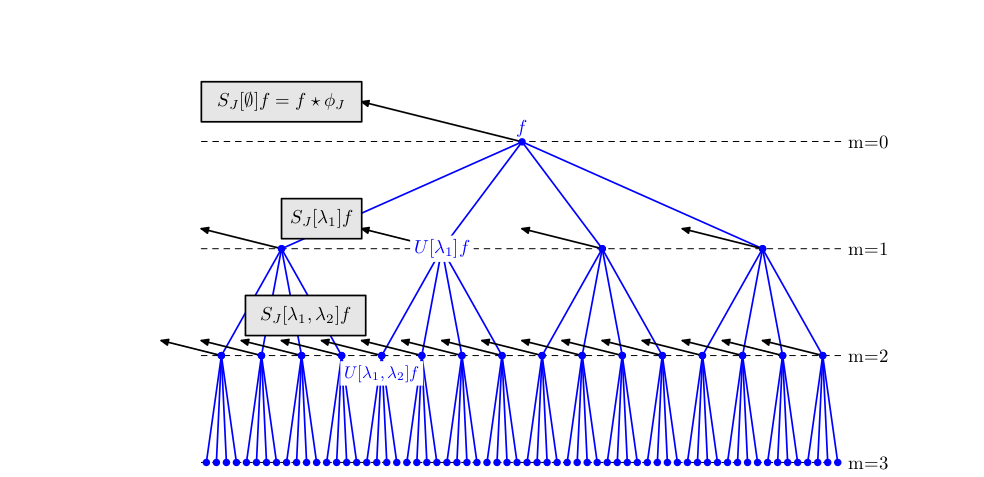
\includegraphics[width=0.8\textwidth]{img/ScatteringPropagator.png}
  \caption{Un PD $U_J$ aplicado a un punto de una señal $f(x)$ calcula $U[\lambda_1]f(x)=|f(x)\ast \psi_{\lambda_1}|$ y como salida a la capa $m=0$ se promedian los coeficientes que han dado $0$ (por tener $2^j<2^-j$) obteniendo como salida $S_J[\emptyset]f(x)=f(x)\ast \phi_{2^J}$ (como se puede ver en la flecha negra). Después se aplica de nuevo $U_J$ a cada coeficiente $U[\lambda_1]f(x)$ del paso anterior ($m=1$) $U[\lambda_1,\lambda2]f(x)$ obteniendo como salida $S_J[\lambda_1]f(x)=U[\lambda_1]f(x) \ast \phi_{2^J}$. Se repite este proceso de manera recursiva para cada coeficiente $U[p]f(x)$ y obteniendo como resultado $S_J[p]f(x)=U[p]f(x) \ast \phi_{2^J}$. }
  \label{fig:scattering_propagator}
\end{figure}


\subsection{Diferencias y similitudes con una CNN}


Las operaciones de la transformada de dispersión que hemos descrito siguen la estructura general de la red neuronal convolucional introducida por LeCun \cite{lecun2015deep}, pues se describen las redes convolucionales como una cascada de convoluciones (la transfomada de ondeletas $W[\lambda]$) y capas de "pooling" que usan funciones no lineales (el operador módulo $M[\lambda]$), las cuales se representan en este modelo como módulos de números complejos. También se puede considerar como un operador de \entrecomillado{pooling} la función $\phi_{2^J}$ que se emplea para agregar coeficientes y contruir un operador invariante.

\medskip

\noindent Las redes neuronales convolucionales han sido empleadas con mucho éxito en tareas de reconocimiento de objetos o personas y usan normalmente Kernels que no son predefinidos, sino que se aprenden mediante la técnica de back-propagation al entrenar la red, en cambio, en la modelización que se ha presentado las ondeletas que usamos son prefijadas y no se aprenden.

\medskip

\noindent Siguiendo con las similitudes entre ambos modelos, si $p$ es un camino de longitud $m$, entonces a $S_J[p] f(x)$ se le denomina coeficiente de orden $m$ a escala $2^J$, que en el caso de una CNN,equivaldría al tensor formado por los mapas de activación tras la convolución con el kernel de la capa $m$ de la red. 

\medskip


\subsection{Relación con herramientas clásicas de visión por computador}
\noindent Por otro lado, la modelización  con los algoritmos clásicos de visión por computador como \textbf{SIFT}  \cite{DistinctiveImageFeatures} para calcular puntos de interés en imágenes. Así, con la ondeletas apropiadas, los coeficientes de primer orden $S[\lambda_1] f$ serían equivalentes a los coeficientes del algoritmo. De hecho, en el artículo sobre el descriptor DAISY \cite{Daisy} se muestra cómo esos coeficientes son aproximados por $S_J[2^j r] f= | f \ast \psi_{2^j r} | \ast \phi_{2^J}(x)$, dónde $\psi_{2^j r}$ es la derivada parcial de una Gaussiana calculada en imagen de escala $2^j$ de mayor calidad, para 8 rotaciones distintas $r$. El filtro para promediar $\phi_{2^J}$ es un filtro Gaussiano escalado.


\subsection{Operador no expansivo.}

\noindent El propagador $U_Jf=\lbrace A_Jf, \left(\left| W[\lambda]f\right|\right)_{\lambda\in\Lambda_J} \rbrace$ es no expansivo, porque la transformada de ondas $W_J$ es unitaria pues cumple las hipótesis de la \autoref{unitario} y el módulo no es expansivo en el sentido de que $||a|-|b||\leq |a-b|$ para cualquier $(a,b)\in \mathbb{C}^2$. Esto es válido tanto si $f$ es real o compleja. Como consecuencia: 

\begin{align*} 
    ||U_J f-U_J h||^2 &= ||A_J f-A_J h||^2+\sum_{\lambda\in\Lambda_J} \left\| |W[\lambda]f|-|W[\lambda]h| \right\|^2 \\
    &\leq \left| \left| W_J f- W_J h \right| \right|^2 \leq ||f-h||^2
\end{align*}

\noindent Al ser $W_J$ unitaria, tomando la función nula $h=0$ y siguiendo el mismo razonamiento anterior, también se comprueba que $||U_J f||=||f||$ por lo que el operador $U_J$ preserva la norma.

\medskip

\noindent Para todo conjunto de caminos $\Omega$, las normas de $S_J[\Omega]f$ y $U[\Omega]f$ son: 

$$\left|\left| S_J[\Omega]f \right|\right|^2=\sum_{p\in\Omega} \left|\left| S_J[p]f\right|\right|^2 \;\; y \;\; \left|\left|U[\Omega]f\right|\right|^2=\sum_{p\in\Omega} \left|\left| U[p]f\right|\right|^2$$

\noindent Como $S_J[\mathcal{P}_J]$ itera en $U_J$, que es no expansivo, la siguiente proposición prueba que $S_J[\Omega]f$ es también no expansivo. 

\begin{proposicion} \label{proposicion::NoExpansiva}
La transformada de dispersión de ventana es no expansiva: 

\begin{equation}
  \forall (f,h)\in L^2(\mathbb{R}^d)^2 \;\; ||S_J[\mathcal{P}_J]f-S_J[\mathcal{P}_J]h|| \leq ||f-h||
\end{equation}
\end{proposicion}

\begin{proof}
Como $U_J$ es no expansiva, partiendo de \eqref{eq::1.5} que nos dice: 
$$U_J U[\Lambda_J^m]=\lbrace S_J[\Lambda_J^m]f,(U[\Lambda_J^{m+1}]f)_{\lambda\in\Lambda_J}\rbrace,$$

se tiene que:

\begin{align*}
    ||U[\Lambda_J^m]f-U[\Lambda_J^m]h||^2 &\geq ||U_J U[\Lambda_J^m]f-U_J U[\Lambda_J^m]h||^2 \\
    & = ||S_J[\Lambda_J^m]f - S_J[\Lambda_J^m]h||^2 + ||U[\Lambda_J^{m+1}]f-U[\Lambda_J^{m+1}]h||^2.
\end{align*}

\medskip

\noindent Si ahora sumamos en $m$ cuando tiende a $\infty$ se obtiene que: 

\begin{align*}
  \sum_{m=0}^{\infty}||U[\Lambda_J^m]f-U[\Lambda_J^m]h||^2 &\geq \sum_{m=0}^{\infty} ||S_J[\Lambda_J^m]f - S_J[\Lambda_J^m]h||^2 + \sum_{m=0}^{\infty} ||U[\Lambda_J^{m+1}]f-U[\Lambda_J^{m+1}]h||^2,\\
\end{align*}

\noindent que equivale a:

\begin{align*}
  \sum_{m=0}^{\infty}||U[\Lambda_J^m]f-U[\Lambda_J^m]h||^2 - \sum_{m=0}^{\infty} ||U[\Lambda_J^{m+1}]f-U[\Lambda_J^{m+1}]h||^2 &\geq \sum_{m=0}^{\infty} ||S_J[\Lambda_J^m]f - S_J[\Lambda_J^m]h||^2\\
\end{align*}

\noindent Si ahora nos fijamos en el lado izquierdo de la desigualdad, se cancelan todos los términos salvo $m=0$, y teniendo en cuenta que $\Lambda^0_J=\emptyset$ queda: 

\begin{align*}
  \sum_{m=0}^{\infty}||U[\Lambda_J^0]f-U[\Lambda_J^0]h||^2 &= \sum_{m=0}^{\infty}||U[\emptyset]f-U[\emptyset]h||^2 = || f - h ||^2 \\
\end{align*}

\noindent Por otro lado, se tiene que

\begin{align*}
  \sum_{m=0}^{\infty} ||S_J[\Lambda_J^m]f - S_J[\Lambda_J^m]h||^2 = ||S_J[\mathcal{P}_J]f - S_J[\mathcal{P}_J]h||^2. \\
\end{align*}

\noindent Luego hemos probado que 

$$||S_J[\mathcal{P}_J]f - S_J[\mathcal{P}_J]h||^2 \leq || f - h ||^2$$

\noindent y por lo tanto que la transfomada de dispersión de ventana es no expansiva. \qedhere
\end{proof}

\subsection{Conservación de la norma.}

En la \autoref{ch:seccion12} se obtuvo que cada coeficiente $U[\lambda]f=|f \ast \psi_\lambda|$ capturaba la energía de frecuencia de $f$ en una banda de frecuencia cubierta por $\widehat{\psi}_\lambda$ y propagaba dicha energía a frecuencias decrecientes, este hecho lo demuestra el siguiente teorema, mostrando que toda la energía del propagador de dispersión alncanza la frecuencia mínima $2^J$ y es atrapada por el filtro paso bajo $\phi_ {2^J}$. La energía propagada tiende a $0$ conforme se incrementa la longitud del camino, y el teorema implica que $||S_J[\mathcal{P}_J]f||=||f||$. Esto se aplica también a funciones complejas en caminos negativos.

\medskip

\noindent Para la demostración de la conservación de la norma necesitamos unos resultados previos: 

\begin{lema} \label{lema::Cota_inferior}
  Si $h$ es una funciones tal que $h\geq 0$ entonces $\forall f \in L^2(\mathbb{R}^d)$: 
  
  \begin{equation}
    |f \ast \psi_\lambda | \ast h \geq \sup_{\eta \in \mathbb{R}^d} |f\ast \psi_\lambda \ast h_\eta | \; \; con \; h_\eta=h(x)e^{i\eta x}
  \end{equation}
\end{lema}
  
\begin{proof}
  
  \begin{align*}
      |f \ast \psi_\lambda | \ast h (x) &= \int \left| \int f(v)\psi_\lambda(u-v)dv \right| h(x-u)du \\
      &=\int \left | \int f(v) \psi_\lambda(u-v) e^{i\eta(x-u)} h(x-u) dv \right| du \\
      &\geq \left | \int \int f(v) \psi_\lambda(u-v) e^{i\eta(x-u)} h(x-u) dv du \right| = \\
      &= \left | \int f(v) \int  \psi_\lambda(x-v-u')h(u') e^{i\eta u'}  du' dv \right| \\
      &= \left | \int f(v) \psi_\lambda \ast h_\eta(x-v) dv \right| = |f\ast \psi_\lambda \ast h_\eta|
  \end{align*}

  \noindent Dónde se ha usado el cambio de variabel $u'=x-u$ con $J=1$.
\end{proof}

\noindent A continuación definimos el concepto de \entrecomillado{ondeleta admisible:}
\begin{definicion}
  Una ondeleta de dispersión se dice que es admisible si existe $\eta \in \mathbb{R}^d$ y una función $\rho \geq 0$, con $|\widehat{\rho}(\omega)| \leq |\widehat{\phi}(2\omega)|$ y $\widehat{\rho}(0)=1$, tal que la función: 

\begin{equation}\label{eq::1.6}
  \widehat{\Psi}(\omega)=|\widehat{\rho}(\omega - \eta)|^2 - \sum_{k=1}^{+\infty} k(1-|\widehat{\rho}(2^{-k}(\omega - \eta))|^2)
\end{equation}
  
\noindent satisface: 
\begin{equation} \label{eq::1.7}
  \alpha= \inf_{1\leq|w|\leq2} \sum_{j=-\infty}^{\infty} \sum_{r\in G} \widehat{\Psi} (2^{-j}r^{-1}\omega)|\widehat{\psi}(2^{-j}r^{-1}\omega)|^2>0.
\end{equation}

\end{definicion}

\noindent Con esta definición en mente podemos comprobar que se da el siguiente lema que demuestra que el propagador dispersa la energía progresivamente hacia bajas frecuencias.

\begin{lema} \label{lema::Admisibilidad}
Si \eqref{eq::1.7} se satisface y 

\begin{equation}
  ||f||_w^2=\sum_{j=0}^\infty \sum_{r\in G^+} j ||W[2^j r] f||^2 < \infty
\end{equation}

\noindent Entonces se tiene: 

\begin{equation}\label{eq::1.9}
  \frac{\alpha}{2}||U[\mathcal{P_J}]f||^2 \geq \max (J+1,1) ||f||^2 + ||f||_w^2.
\end{equation}

\end{lema}

\medskip

\noindent La demostración de lema se encuentra en el apéndice A de \cite{GroupInvariantScattering}.

\medskip

\noindent Con todos estos resultados podemos presentar el principal teorema de esta sección, que nos dará como resultado la preservación de la norma del operador de ventana:


\begin{teorema} \label{teoremaOndeletasAdmisibles}
\noindent Si las ondeletas son admisibles, entonces para toda $f\in L^2(\mathbb{R}^d)$
\begin{equation}
  \lim_{m\rightarrow\infty} ||U[\Lambda_J^m]f||^2=\lim_{m\rightarrow\infty} \sum_{n=m}^{\infty} ||S_J[\Lambda_J^n]f||^2=0
\end{equation}

y

\begin{equation}
  ||S_J[\mathcal{P_J}]f||=||f||
\end{equation}

\end{teorema}

\begin{proof}
  Esta demostración tiene dos partes, la primera consistirá en demostrar que la condición \eqref{eq::1.6} implica que $\lim_{m\rightarrow \infty} ||U[\Lambda_J^m]f||^2=0$. 
  
  \medskip

  \noindent La clave de esto reside en el \autoref{lema::Cota_inferior}, que nos da una cota inferior de $|f\ast\psi_\lambda|$ convolucionada con una función positiva. La clase de funciones para las que $||f||_w < \infty$ es una clase logarítmica de Sobolev correspondiente a funciones que tienen un módulo promedio continuo en $L^2(\mathbb{R}^d)$. Como 

  $$ || U[\mathcal{P}_J]f ||^2= \sum_{m=0}^{+\infty} ||U[\Lambda_J^m]f||^2,$$

  \noindent si $||f||_w < \infty$ entonces \eqref{eq::1.9} implica que $\lim_{m\rightarrow\infty}||U[\Lambda_J^m]f||= 0$. Este resultado se extiende en $L^2(\mathbb{R}^d)$ por densidad. Como $\phi \in L^1(\mathbb{R}^d)$ y $\widehat{\phi}(0)=1$, cualquier $f\in L^2(\mathbb{R}^d)$ satisface $\lim_{n\rightarrow - \infty} ||f-f_n||=0$, dónde $f_n=f \ast \phi_{2^n}$ y $\phi_{2^n}=2^{-nd} \phi(2^{-n}x)$. Se demuestra por tanto que $\lim_{m\rightarrow \infty} ||U[\Lambda_J^m]f_n||=0$ viendo que $||f_n||_w < \infty$. De hecho, 


  \begin{align*}
      ||W[2^jr]f_n||^2 &= \int |\widehat{f}(\omega)|^2 |\widehat{\phi}(2^n \omega)|^2 |\widehat{\psi}(2^{-j}r^{-1}\omega)|^2 d\omega \\
      &\leq C 2^{-2n-2j} \int |\widehat{f}(\omega)|^2 d\omega,
  \end{align*}

  \noindent porque $\psi$ hay un momento en que desaparece entonce $|\widehat{\psi}(\omega)=O(|\omega|)$, y las derivadas de $\phi$ están en $L^1(\mathbb{R}^d)$ luego $|\omega||\widehat{\phi}\omega|$ están acotadas. Por lo que se tiene que $||f_n||_w < \infty$.

  \medskip

  \noindent Como $U[\Lambda^m]$ es no expansiva, $||U[\Lambda_J^m]f-U[\Lambda_J^m]f_m|| \leq ||f - f_n||$, por lo que 

  $$||U[\Lambda_J^m]f|| \leq || f-f_n|| + ||U[\Lambda_J^m]f_n||.$$

  \noindent Como $\lim_{n\rightarrow -\infty}||f-f_n||=0$ y $\lim_{m\rightarrow\infty}||U[\Lambda_J^m]f_n||=0$ tenemos que 

  $$\lim_{m\rightarrow\infty} ||U[\Lambda_J^m]f||^2=0$$

  \noindent para toda $f \in L^2(\mathbb{R}^d)$. 

  \medskip

  \noindent \textbf{En segundo lugar} vamos a ver que las siguientes expresiones son equivalentes: 
  \begin{align*}
    \lim_{m\rightarrow \infty} ||U[\Lambda_J^m]f||^2=0 \iff \lim_{m\rightarrow\infty} \sum_{n=m}^{\infty} ||S_J[\Lambda_J^n]f||^2=0 \iff ||S_J[\mathcal{P_J}]f||^2 = ||f||
  \end{align*}

  En primer lugar probamos que 
  $$\lim_{m\rightarrow \infty} ||U[\Lambda_J^m]f||^2=0 \iff \lim_{m\rightarrow\infty} \sum_{n=m}^{\infty} ||S_J[\Lambda_J^n]f||^2=0$$
  
  \noindent Como $||U_J h||=||h|| \; \forall h \in L^2(\mathbb{R}^d)$ y $U_J U[\Lambda_J^n]f=\lbrace S_J[\Lambda_J^n]f,U[\Lambda_J^{n+1}]\rbrace$,

 \begin{equation} \label{eq::1.8}
  ||U[\Lambda_J^n]f||^2=||U_JU[\Lambda_J^n]f||^2=||S_J[\Lambda_J^n]f||^2+||U[\Lambda_J^{n+1}]f||^2. 
 \end{equation}

  \noindent Sumando en $m\leq n < \infty$ se obtiene : 
  
  \begin{align*}
    \sum_{n=m}^\infty ||U[\Lambda_J^n]f||^2=&\sum_{n=m}^\infty ||S_J[\Lambda_J^n]f||^2 + \sum_{n=m}^\infty||U[\Lambda_J^{n+1}]f||^2 \\
    \Big\Updownarrow \\
    \sum_{n=m}^\infty ||U[\Lambda_J^n]f||^2 -& \sum_{n=m}^\infty||U[\Lambda_J^{n+1}]f||^2 =\sum_{n=m}^\infty ||S_J[\Lambda_J^n]f||^2  \\
  \end{align*}
  
  \noindent En el término de la izquierda se anulan entre si todos los sumandos salvo $n=m$, luego queda: 

  \begin{align*}
    ||U[\Lambda_J^m]f||^2 =\sum_{n=m}^\infty ||S_J[\Lambda_J^n]f||^2  \\
  \end{align*}
  \noindent Y tomando límites cuando $m\rightarrow \infty$
  \begin{align*}
    \lim_{m\rightarrow \infty}||U[\Lambda_J^m]f||^2 =\lim_{m\rightarrow \infty}\sum_{n=m}^\infty ||S_J[\Lambda_J^n]f||^2  \\
  \end{align*}
  \noindent Llegados a este punto se puede apreciar claramente que
  
  $$Si \; \; \lim_{m\rightarrow \infty} ||U[\Lambda_J^m]f||^2=0 \implies \lim_{m\rightarrow\infty} \sum_{n=m}^{\infty} ||S_J[\Lambda_J^n]f||^2=0$$

  \noindent Y el recíproco también es cierto, luego ambas expresiones son equivalentes.

  \medskip

  \noindent Por otro lado, sumando en \eqref{eq::1.8} para $0\leq n < m$ se obtine:

  \begin{align*}
    \sum_{n=0}^{m-1} ||U[\Lambda_J^n]f||^2=&\sum_{n=0}^{m-1} ||S_J[\Lambda_J^n]f||^2 +\sum_{n=0}^{m-1}||U[\Lambda_J^{n+1}]f||^2 \\
    \Big\Updownarrow \\
    \sum_{n=0}^{m-1} ||U[\Lambda_J^n]f||^2 -& \sum_{n=0}^{m-1}||U[\Lambda_J^{n+1}]f||^2 = \sum_{n=0}^{m-1} ||S_J[\Lambda_J^n]f||^2.  \\
  \end{align*}
  
  \noindent En el término de la izquierda se anulan entre si todos los sumandos salvo $n=0$, y teniendo en cuenta que $f=U[\Lambda_J^0]f$ queda:
  
  \begin{equation}
    ||f||^2=\sum_{n=0}^{m-1} ||S_J[\Lambda_J^n]f||^2 + ||U[\Lambda_J^m]f||^2.
  \end{equation}

  \noindent Si ahora tomamos límite cuando $m\rightarrow \infty$ obtenemos: 
  \begin{align*}
    \lim_{m\rightarrow \infty}||f||^2 =\lim_{m\rightarrow \infty}\sum_{n=0}^{m-1} ||S_J[\Lambda_J^n]f||^2 &+ \lim_{m\rightarrow \infty} ||U[\Lambda_J^m]f||^2  \\
    \Big\Updownarrow \\
    ||f||^2 =\sum_{n=0}^{\infty} ||S_J[\Lambda_J^n]f||^2 &+ \lim_{m\rightarrow \infty} ||U[\Lambda_J^m]f||^2  \\
    \Big\Updownarrow \\
    ||f||^2 =||S_J[\mathcal{P_J}]f||^2 &+ \lim_{m\rightarrow \infty} ||U[\Lambda_J^m]f||^2.  \\
  \end{align*}

  \noindent De manera que se puede apreciar claramente que  
  \begin{align*}
    ||f||^2 =||S_J[\mathcal{P_J}]f||^2 + \lim_{m\rightarrow \infty} ||U[\Lambda_J^m]f||^2  = ||S_J[\mathcal{P_J}]f||^2 \iff \lim_{m\rightarrow \infty} ||U[\Lambda_J^m]f||^2=0. \\
  \end{align*}

  \noindent Con lo que queda demostrado el teorema \qedhere
\end{proof}

\subsection{Conclusiones extraidas del teorema}
\noindent La demostración muestra que el propagador dispersa la energía progresivamente a frecuencias menores. La energía de $U[p]f$ se concentra principalmente en los caminos de frecuencia decrecientes $p=(\lambda_k)_{k\leq m}$ para los que $|\lambda_{k+1}|<|\lambda_k|$.


\medskip

\noindent El decrecimiento de $\sum_{n=m}^\infty || S_J[\Lambda_J^n]f||^2$ nos sugiere que podemos descartar todos los caminos de longitud mayor que un cierto $m>0$. De hecho, en tareas de tratamiento de imágenes y audio el decrecimiento numérico de $||S_J[\Lambda_J^n]f||^2$ puede llegar a ser exponencial, lo que conlleva a que en problemas de clasificación, por ejemplo, el de camino se liminte a $m=3$.

\medskip

\noindent El teorema además requiere de una transformada de ondeleta unitaria y admisible que satisfaga la condición de Littlewood-Paley $\beta \sum_{(j,r)\in \mathbb{Z}\times G}|\widehat{\psi}(2^jr\omega)|^2=1$. 

\medskip

\noindent Debe también existir una función $\rho \geq 0$ y un $\eta \in \mathbb{R}^d$ con $|\widehat{\rho}(\omega)|\leq |\widehat{\phi}(2\omega)|$ tal que: 

$$\sum_{(j,r)\in\mathbb{Z}\times G}|\widehat{\psi}(2^jr\omega)|^2|\widehat{\rho}(2^jr\omega-\eta)|^2$$

\noindent sea suficientemente grande para que $\alpha>0$. Esto se puede obtener como se indica en $(2.3)$, con $\psi(x)=e^{i\eta x}\Theta(x)$ y de hecho $\widehat{\psi}=\widehat{\Theta}(\omega-\eta)$, dónde $\widehat{\Theta}$ y $\widehat{\rho}$ tienen su energía concentrada en los mismos dominos de frecuencia, que son bajos.

\endinput